\chapter{Application for Real Materials}
\label{chap:sixth}

\thesisepisrcyear{What is the meaning of life?}{John Doe}{Thoughts}{1971}

\chapterintrobox{This is the introduction paragraph.}

\section{Methylammonium Lead Halide Perovskites}
\label{sec:chap-sixth-first}

\begin{table}
\begin{center}
\begin{tabular}{||c|c|c|c||} 
\hline\hline
Phonon Frequencies (THz) & IR Activity & $\epsilon^{\text{ionic}}_j$ & $\alpha_j$ \\
\hline\hline
4.017 & 0.082 & 0.300 & 0.034 \\
\hline
3.888 & 0.006 & 0.025 & 0.003 \\
\hline
3.531 & 0.054 & 0.254 & 0.031 \\ 
\hline
2.755 & 0.021 & 0.166 & 0.023 \\
\hline
2.438 & 0.232 & 2.308 & 0.336 \\
\hline
2.249 & 0.262 & 3.071 & 0.465 \\
\hline
2.080 & 0.234 & 3.203 & 0.505 \\
\hline
2.034 & 0.062 & 0.893 & 0.142 \\
\hline
1.567 & 0.037 & 0.886 & 0.161 \\
\hline
1.019 & 0.013 & 0.721 & 0.162 \\
\hline
1.002 & 0.007 & 0.402 & 0.091 \\
\hline
0.997 & 0.010 & 0.618 & 0.141 \\
\hline
0.920 & 0.011 & 0.767 & 0.182 \\
\hline
0.801 & 0.002 & 0.156 & 0.040 \\
\hline
0.574 & 0.007 & 1.163 & 0.349 \\
\hline\hline
\end{tabular} \label{table:mapidata}
\caption{Infrared activity, ionic dielectric contribution and decomposed Fr\"ohlich alpha values associated with each of the phonon modes in MAPbI3 taken from Ref~\cite{brivio_lattice_2015}. The effective Fr\"ohlich alpha $\alpha_{\text{eff}} = \sum_j \alpha_j$ is found to be $2.66$ for MAPbI3.}
\end{center}
\end{table}

I have produced a Julia Pluto.jl notebook that uses the multiple phonon theory to evaluate the decomposed Fr\"ohlich $\alpha_j$ components associated with $15$ modes of Methylammonium lead iodide (MAPbI$_3$). The frequencies and infrared activities associated with these modes are listed in Table 1. The decomposed $\alpha_j$ parameters and phonon frequencies $\omega_j$ are then inserted into the variational principle for multiple phonons to obtain a $v$ and $w$ parameter that provide the lowest upper-bound to the exact free energy of the multi-modal polaron system. The two effective phonon frequencies schemes, labelled scheme A and B in~\cite{hellwarth_mobility_1999} (c.f. section 3.6.5), evaluate the Fr\"ohlich alpha for MAPbI$_3$ to be $\alpha = 2.52$ (towards zero temperature the A scheme gives a slightly different value of $2.44$). In comparison, including the ionic contributions of each MAPbI$_3$ phonon modes explicitly produced the decomposed Fr\"ohlich alpha $\alpha_j$ shown in Table 1. From these, I obtain an effective alpha for MAPbI$_3$ of $\alpha_{\text{eff}} = 2.66$ which is only slightly larger than the value predicted by the effective mode A and B schemes. The free energy approximated by the multiple phonon theory is shown in comparison the Hellwarth and Biaggio effective mode theory in Figure \ref{fig:multitheory}a. The two Hellwarth schemes agree for almost all temperatures except for a small deviation towards zero temperature where the A scheme gives a slightly lower value. The multiple phonon theory clearly gives a lower estimate to the free energy of the polaron compared to the Hellwarth theory for all temperatures above roughly $100$K but gives a higher value at lower temperatures and at zero temperature. Figure \ref{fig:multitheory}b shows a comparison between the multiple phonon variational $v$ and $w$ parameters compared to the effective variational parameters from the Hellwarth and Biaggio effective mode theory. The two agree at zero temperature, but the multiple phonon theory predicts larger polaron frequencies at higher temperatures and a smaller different in $v$ and $w$, $v - w$, at all temperatures. 

\begin{figure}[t]
    \centering
    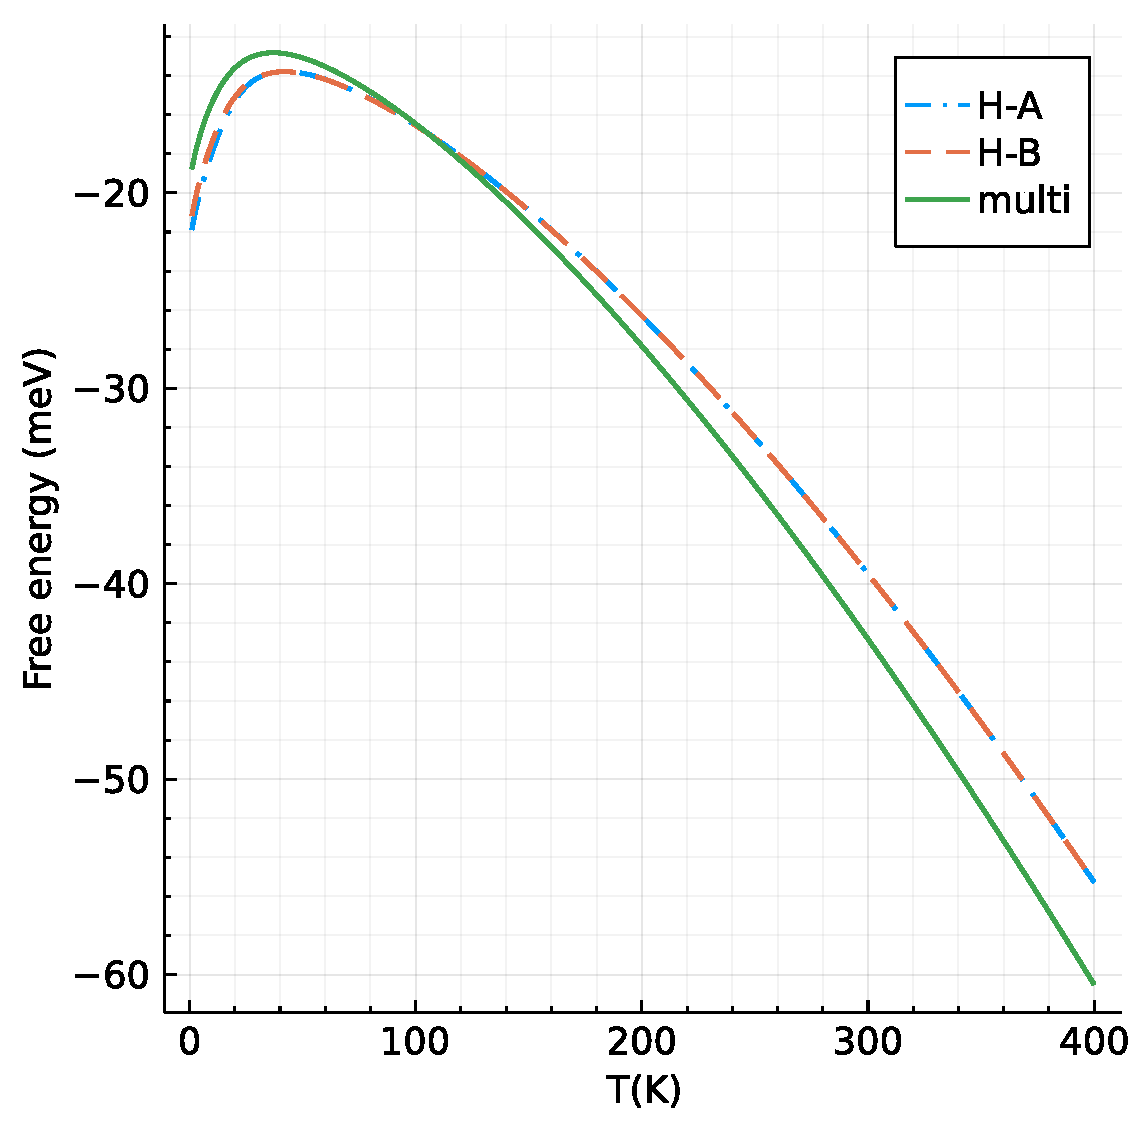
\includegraphics[width=.49\textwidth]{figures/free_energy_temp.pdf}
    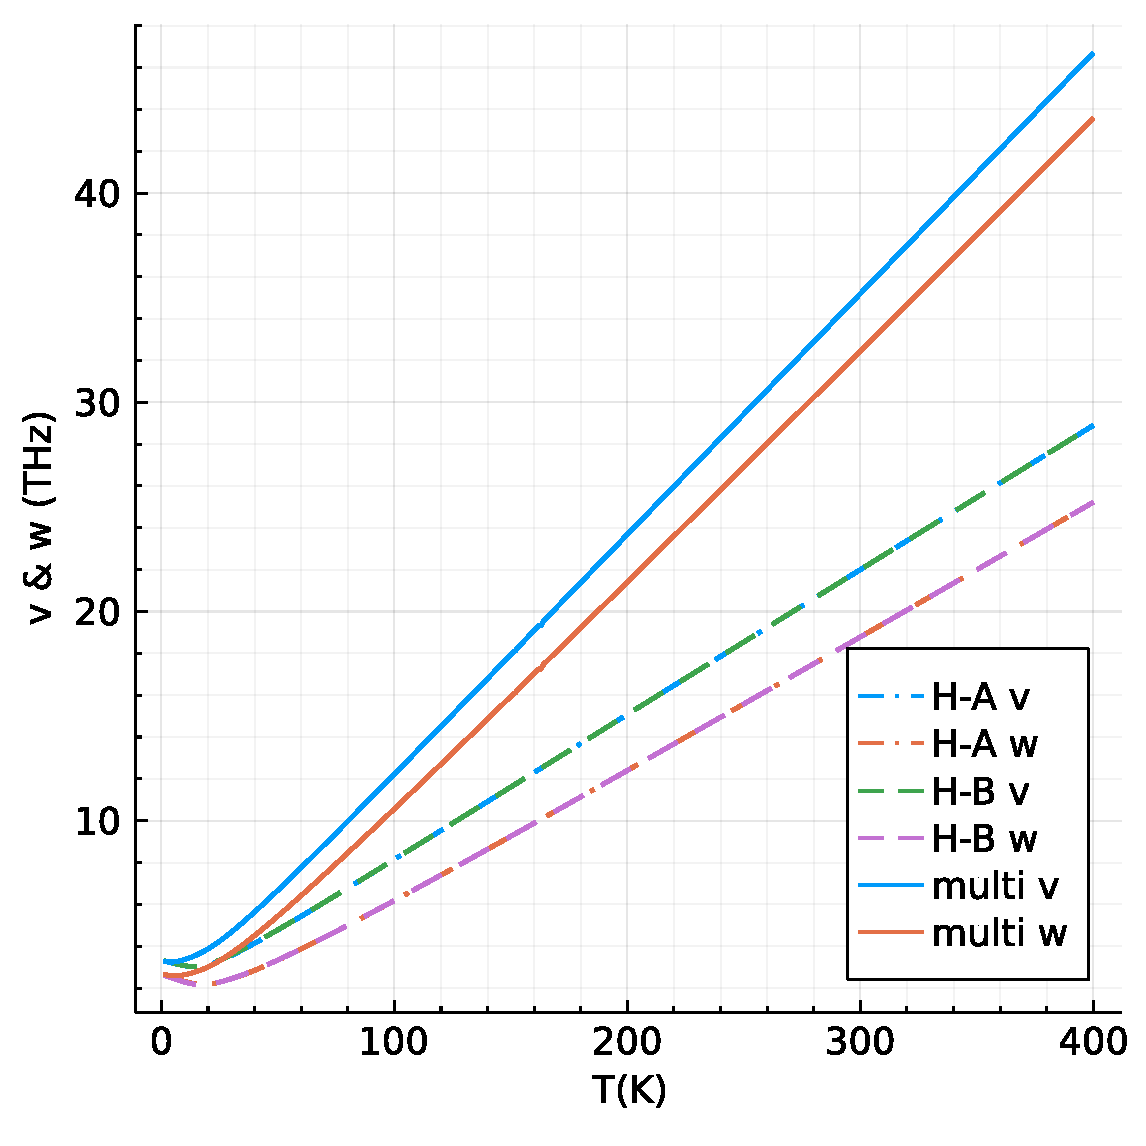
\includegraphics[width=.49\textwidth]{figures/vw_temp.pdf}
    \caption{(left): The free energy of the Hellwarth and Biaggio effective mode A \& B schemes and for the multiple phonon model between $1$K and $400$K. The two Hellwarth schemes agree almost exactly except for a small deviation at low temperatures. The multiple phonon model gives a lower free energy estimate for temperatures above $100$K. (right): The variational parameters $v$ \& $w$ from the Hellwarth and Biaggio effective mode A \& B schemes and the multiple phonon model. The effective mode schemes agree whereas the multiple phonon model gives values larger than the Hellwarth schemes but approaches their values towards zero temperature.}
    \label{fig:multitheory}
\end{figure}

Figures \ref{fig:multicontour} (contour plots) and \ref{fig:multiridge} (ridge-line plots) compare the complex conductivity obtained from the multiple phonon model (left column) to the complex conductivity obtained from the Hellwarth and Biaggio B scheme (right column). The top rows show the real part of the conductivity (i.e. the ac mobility), the middle rows show the imaginary part and the bottom rows show the absolute value. I chose the B scheme over the A scheme because the B scheme involves matching an effective frequency to the full extent of \=Osaka's finite temperature variational principle, so is arguably more accurate. On the other hand, the A scheme produces a temperature-dependent Fr\"ohlich alpha parameter and effective phonon frequency. This is unlike the original Fr\"ohlich alpha and phonon frequency which are independent of temperature. Nonetheless, the two schemes do produce near-identical results for most temperature anyway, except for a slight deviation at very low temperatures. So, a lot of the comparison with the B scheme will be comparable to that of the A scheme too. 

Both the multiple phonon theory and the Hellwarth and Biaggio effective mode theory have similar dc mobilities and high temperature complex conductivities. Likewise, they both possess a broad peak starting around a frequency of $2.03$ THz, which is the effective phonon frequency derived from the B scheme. (At zero temperature, the A scheme gives an effective phonon frequency of $2.17$ THz). The start of the main peak then shifts up in frequency as the temperature increases whilst primarily broadening and flattening. The theories differ in their frequency dependence. Whilst both possess the same main peak starting around $2$ THz, the multiple phonon theory possesses extra peaks below $2$ THz, particular two fairly sharp peaks starting around $0.50$ THz and $1.00$ THz. All of these extra details are washed-out at higher temperatures to leave one main broad peak that has a maximum located at a slightly lower frequency compared to Hellwarth's and Biaggio's theory.

\begin{figure}
    \centering
    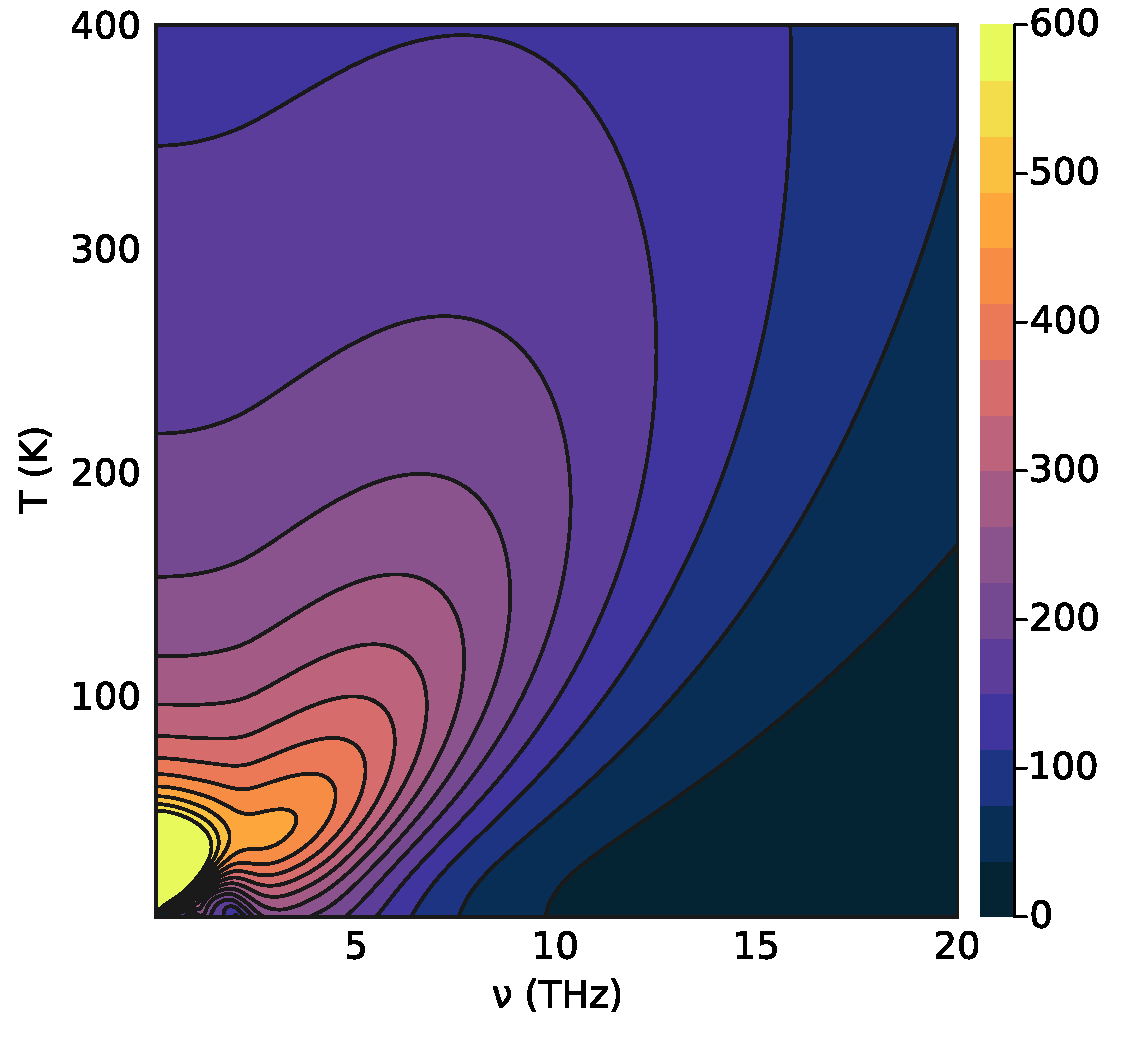
\includegraphics[width=.49\textwidth]{figures/multi_contour_real.pdf}
    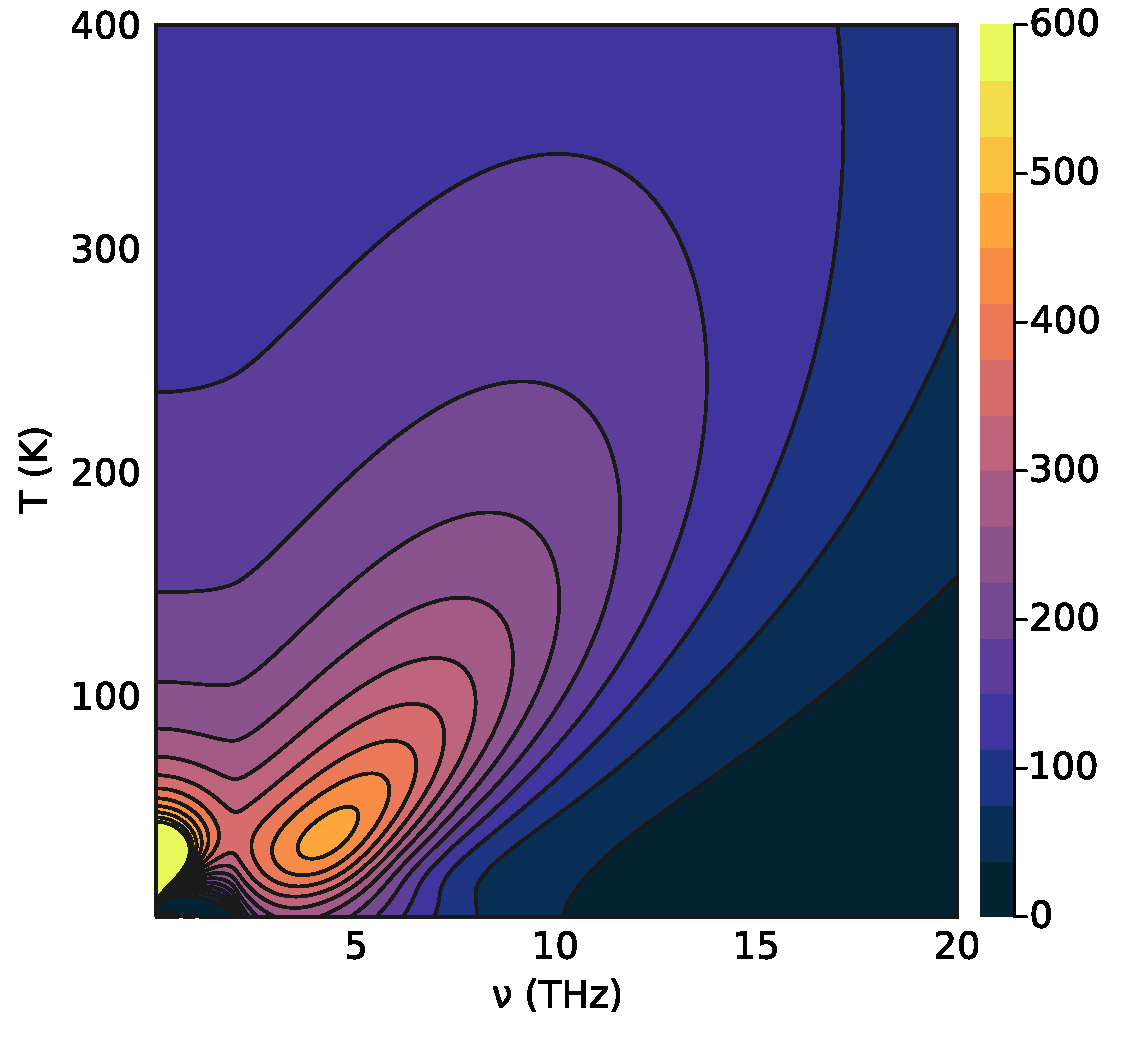
\includegraphics[width=.49\textwidth]{figures/B_contour_real.pdf}
    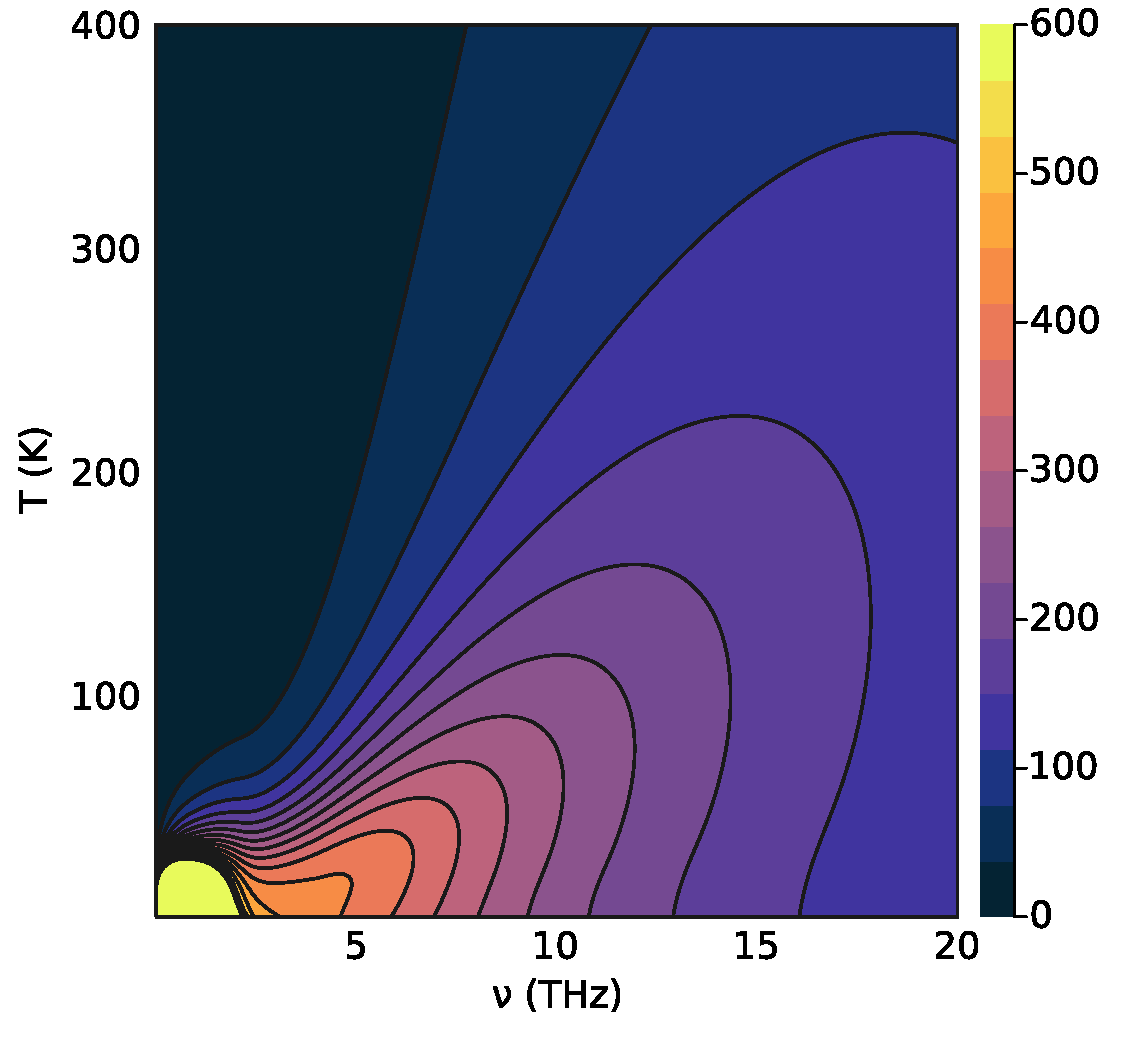
\includegraphics[width=.49\textwidth]{figures/multi_contour_imag.pdf}
    \includegraphics[width=.49\textwidth]{figures/B_contour_imag.pdf}
    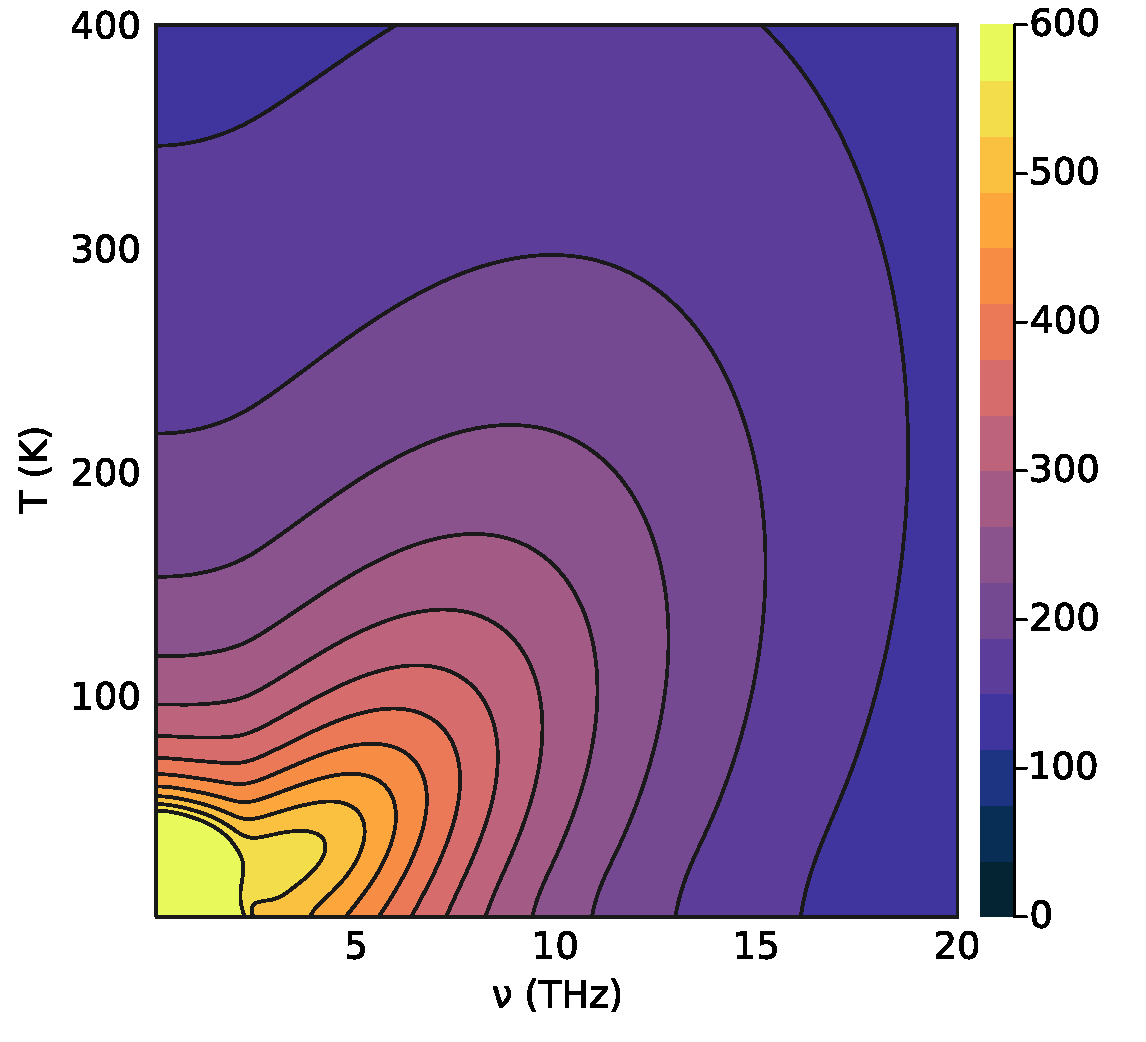
\includegraphics[width=.49\textwidth]{figures/multi_contour_abs.pdf}
    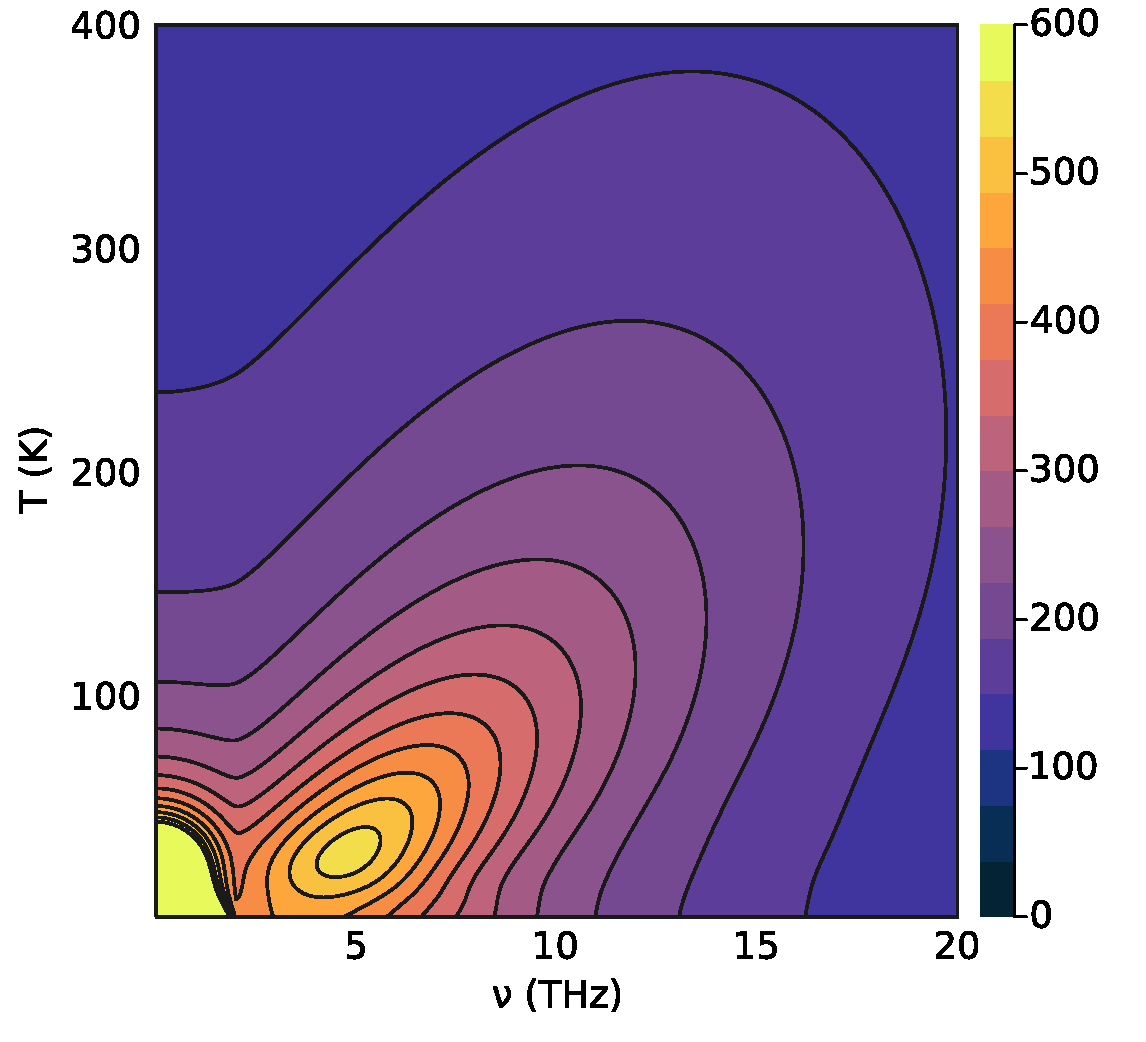
\includegraphics[width=.49\textwidth]{figures/B_contour_abs.pdf}
    \caption{Left: Multiple phonon scheme (a) real conductivity, (c) imaginary conductivity, (e) absolute conductivity. Right: Hellwarth `B' scheme: (b) real conductivity, (d) imaginary conductivity, (f) absolute conductivity.}
    \label{fig:multicontour}
\end{figure}

\begin{figure}
    \centering
    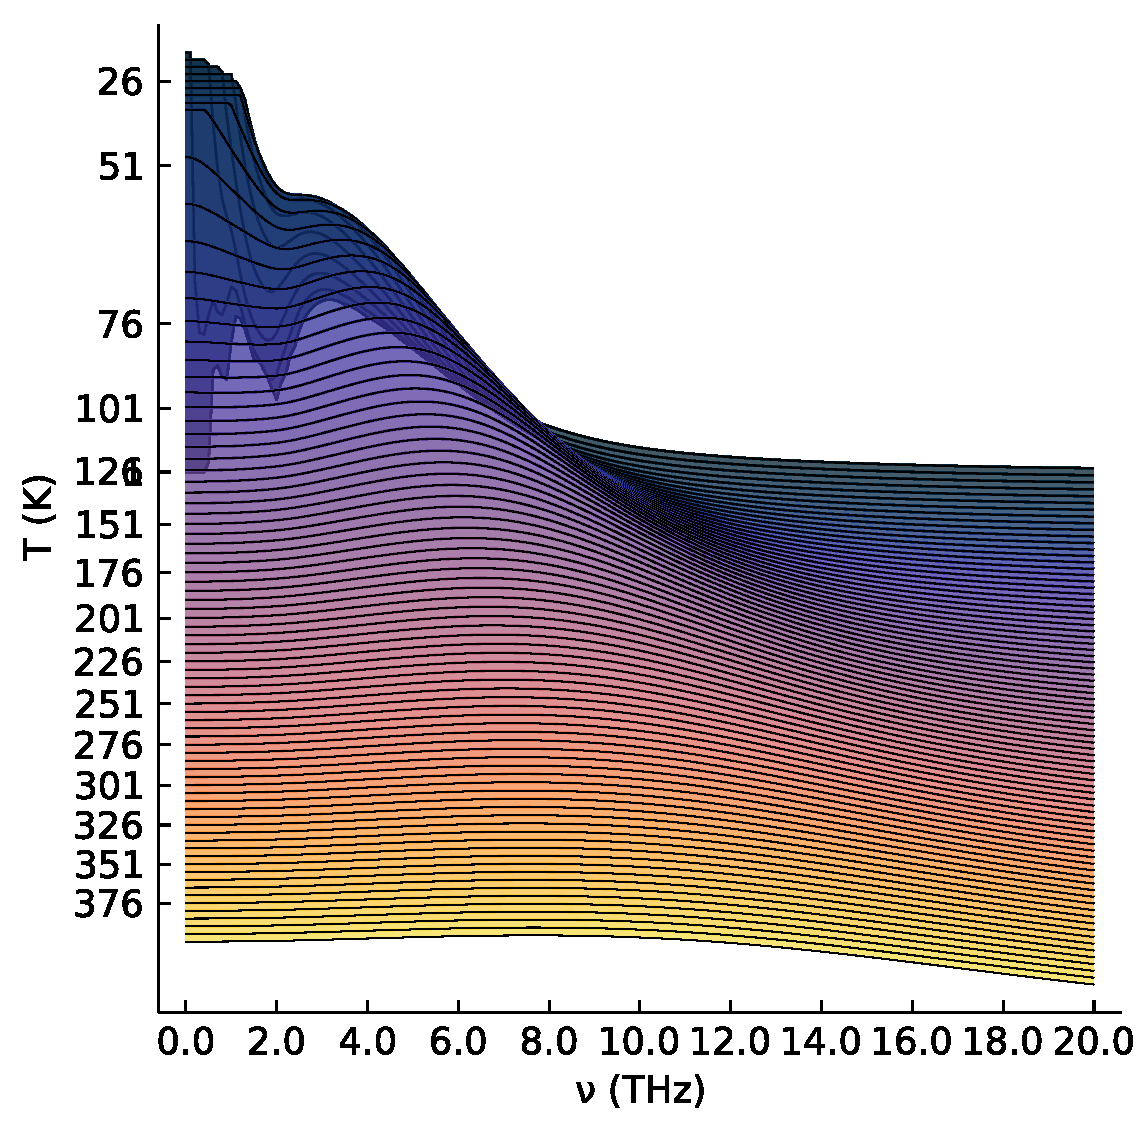
\includegraphics[width=.49\textwidth]{figures/multi_plot_temp_real.pdf}
    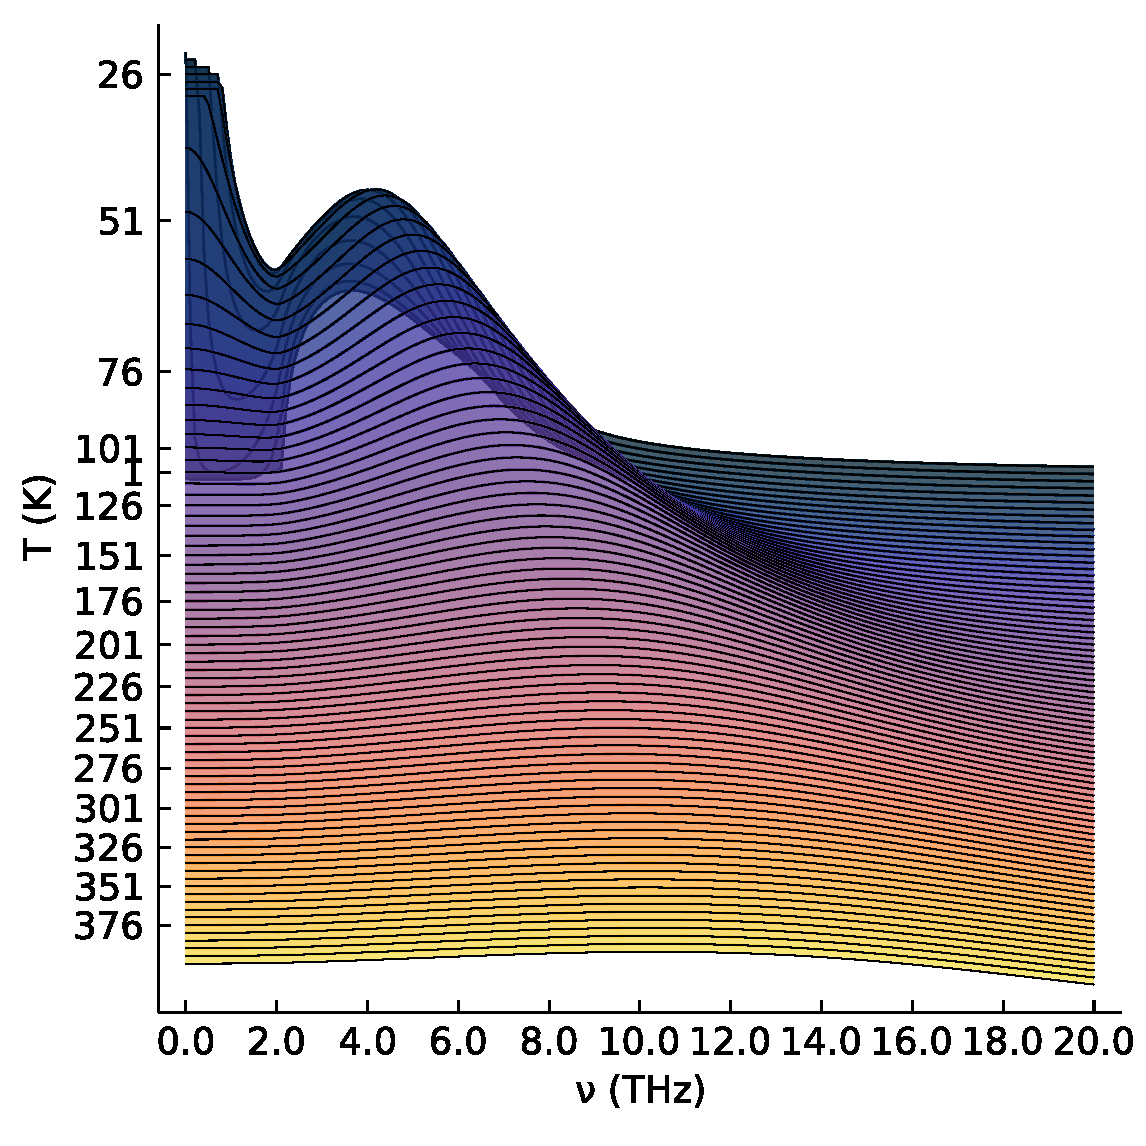
\includegraphics[width=.49\textwidth]{figures/B_plot_temp_real.pdf}
    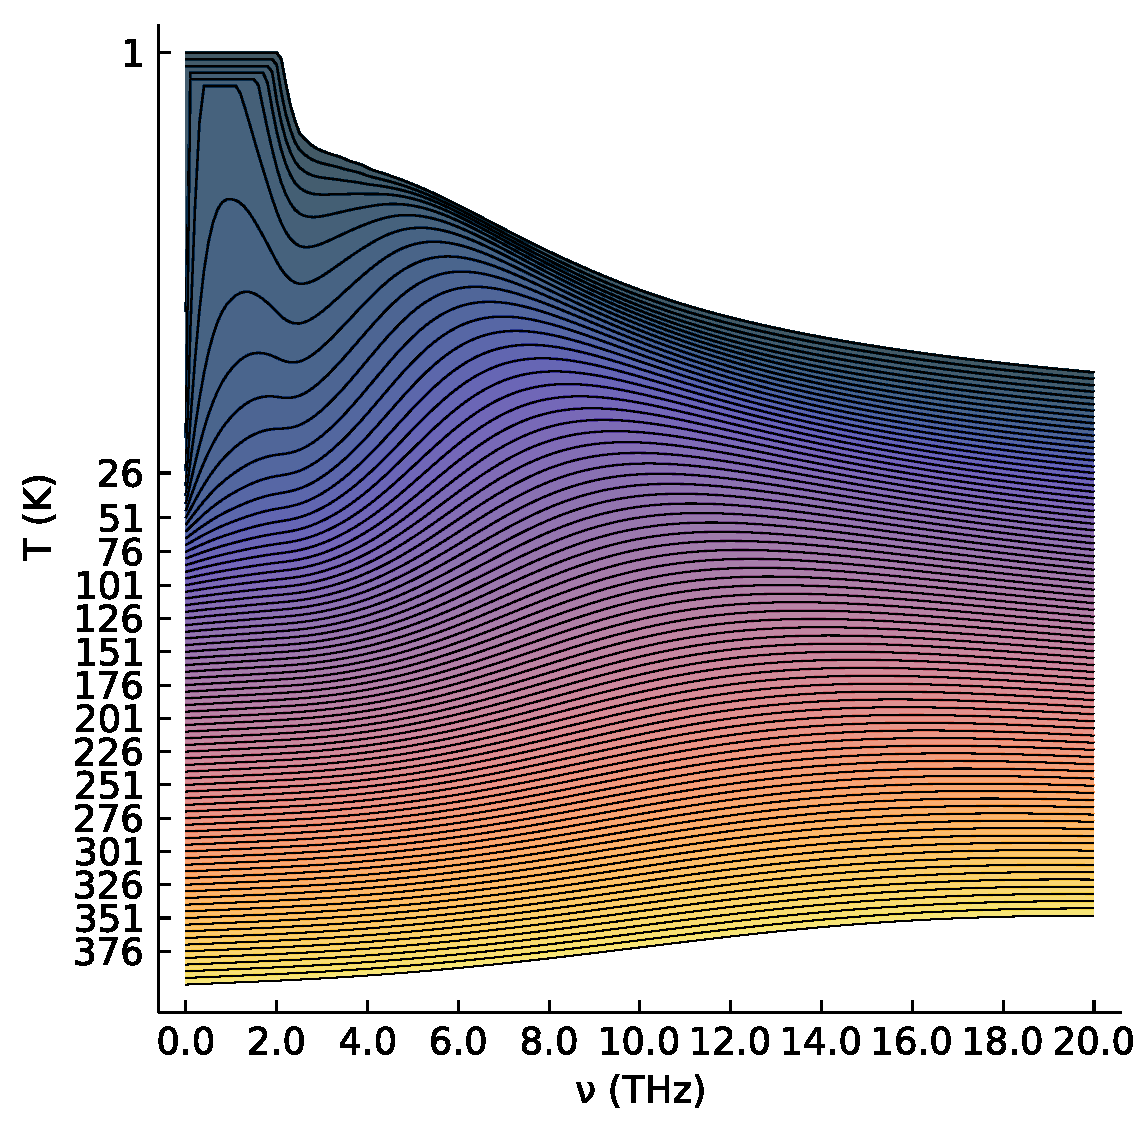
\includegraphics[width=.49\textwidth]{figures/multi_plot_temp_imag.pdf}
    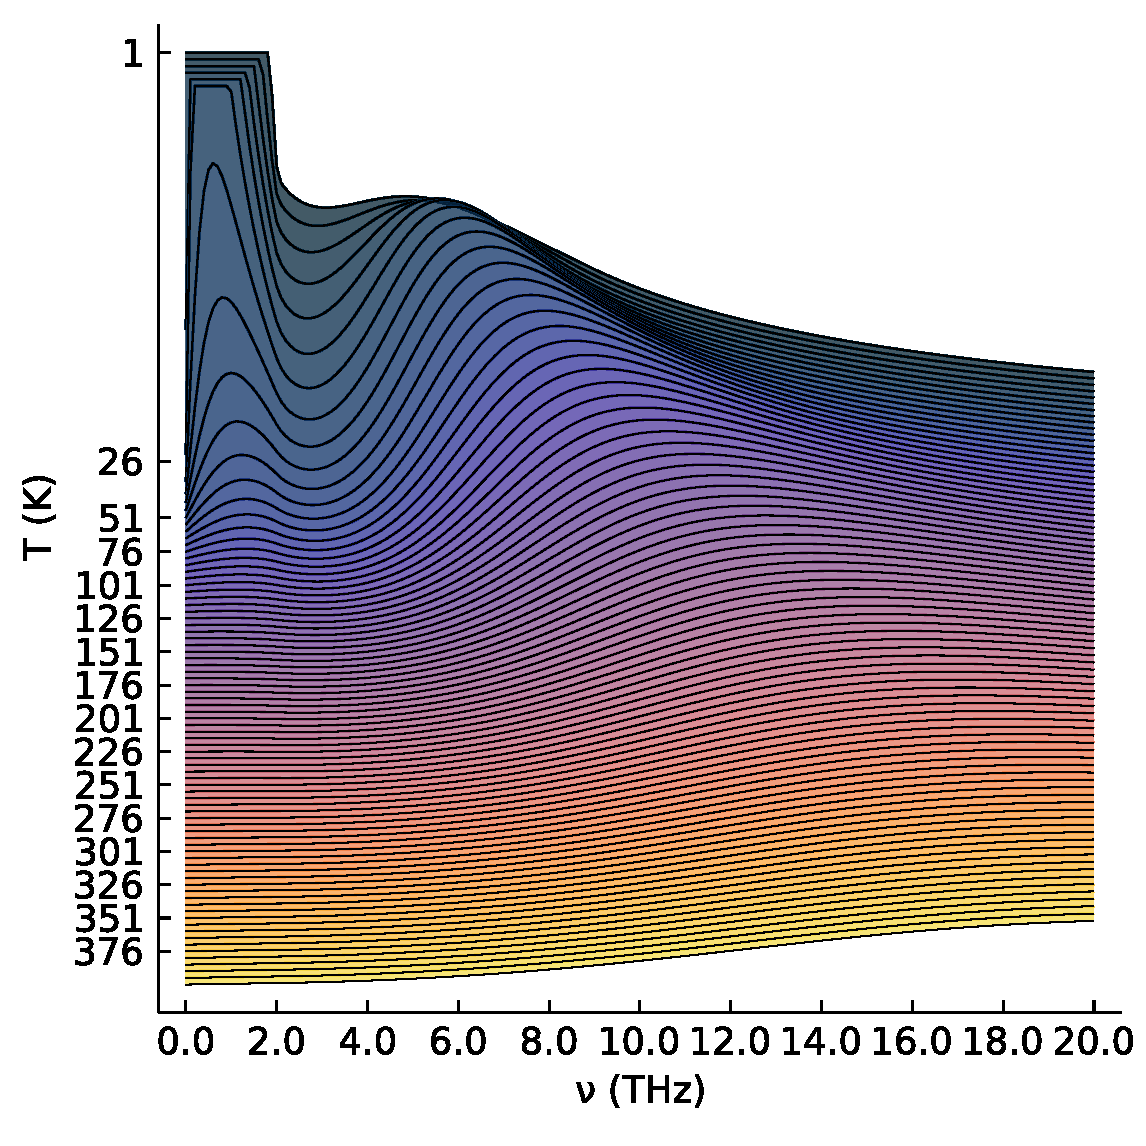
\includegraphics[width=.49\textwidth]{figures/B_plot_temp_imag.pdf}
    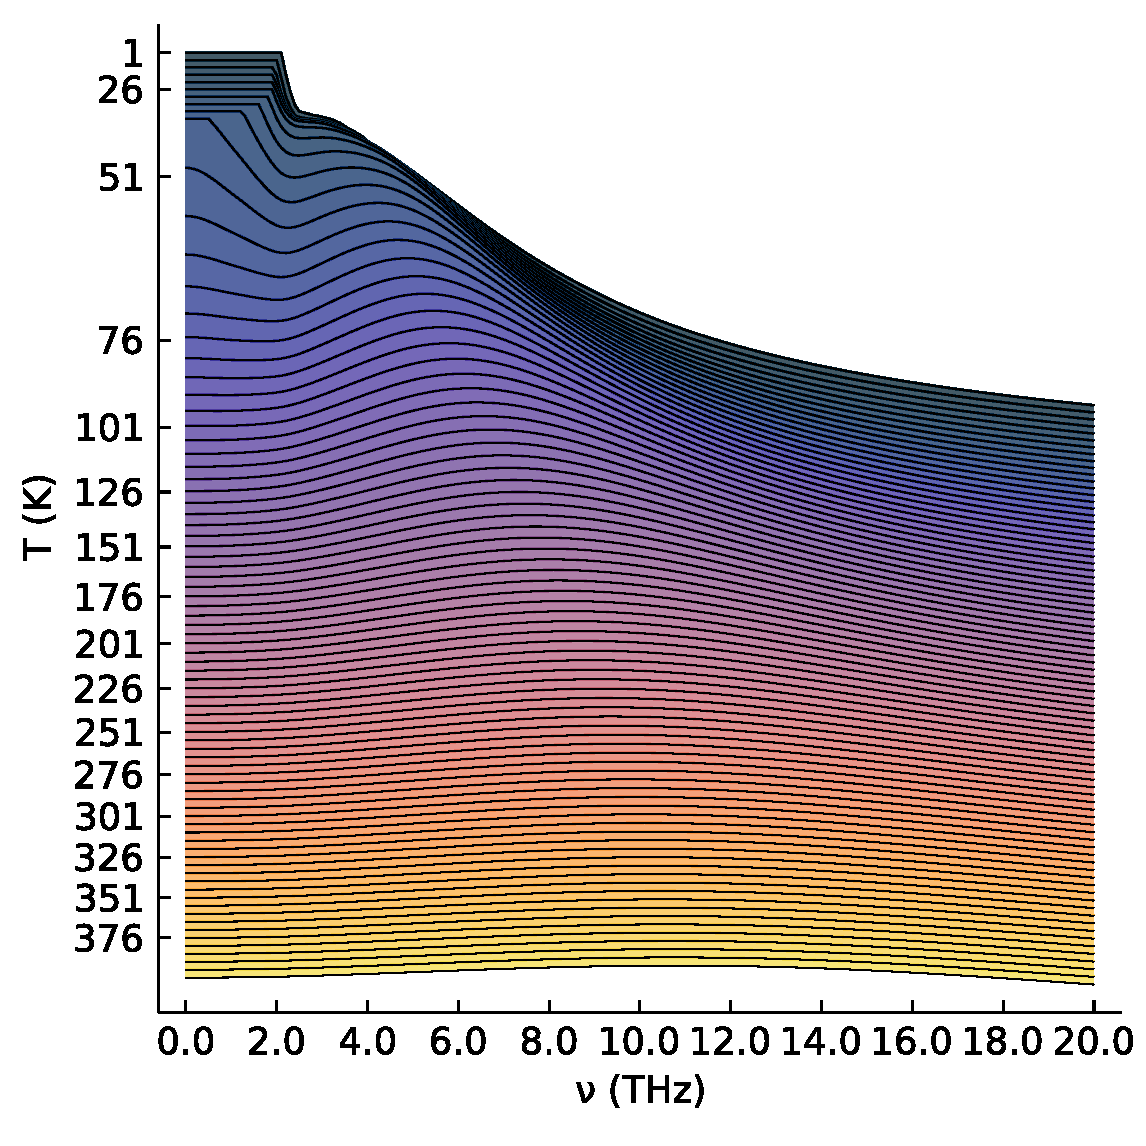
\includegraphics[width=.49\textwidth]{figures/multi_plot_temp_abs.pdf}
    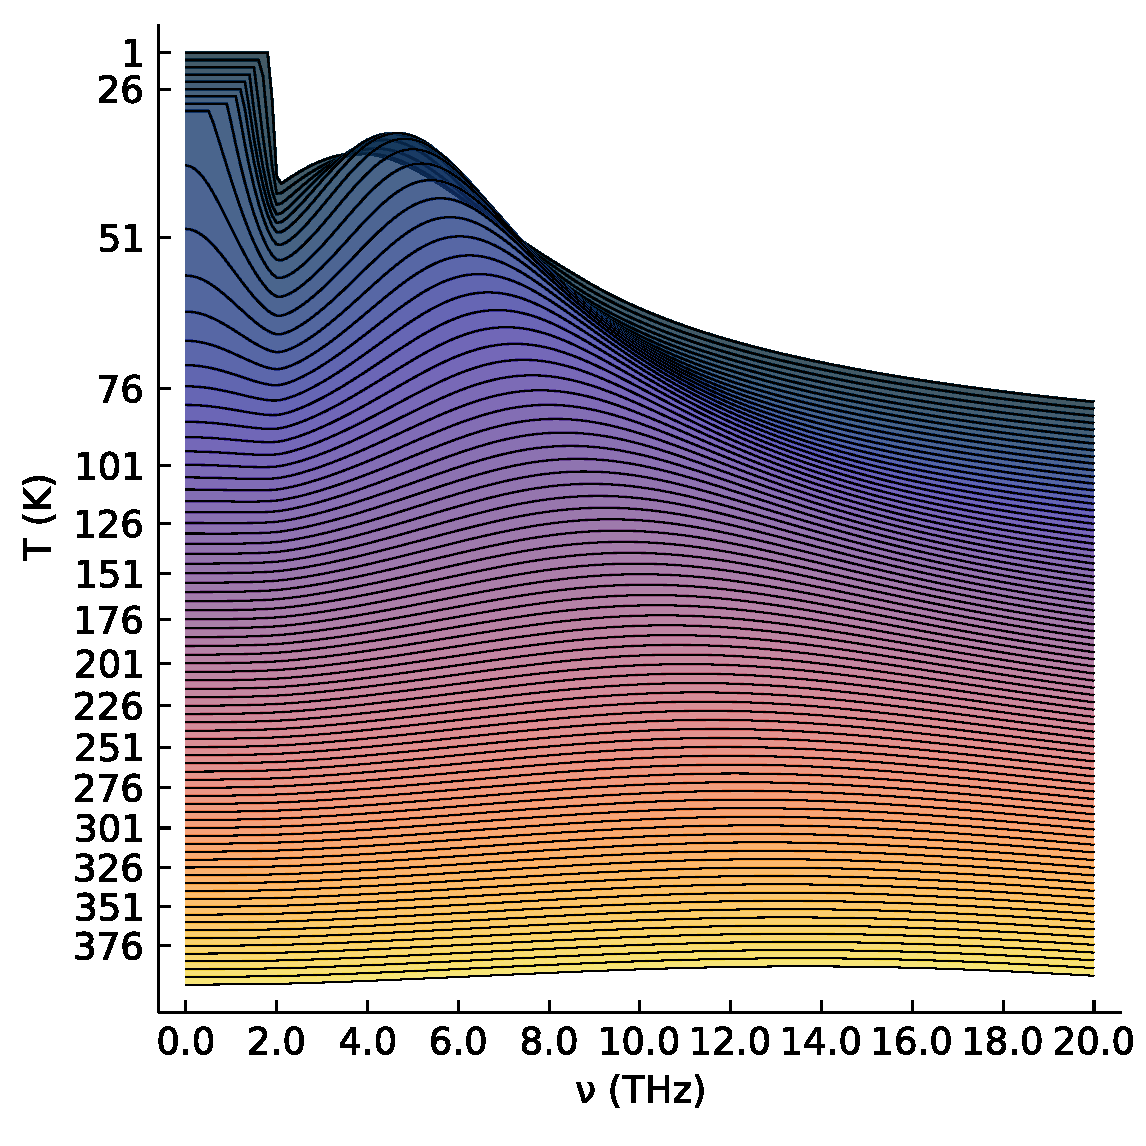
\includegraphics[width=.49\textwidth]{figures/B_plot_temp_abs.pdf}
    \caption{Left: Multiple phonon scheme (a) real conductivity, (c) imaginary conductivity, (e) absolute conductivity. Right: Hellwarth `B' scheme: (b) real conductivity, (d) imaginary conductivity, (f) absolute conductivity. At lower temperatures the conductivity has been cut-off at $600$ to enable us to see the main features.}
    \label{fig:multiridge}
\end{figure}

\begin{figure}
    \centering
    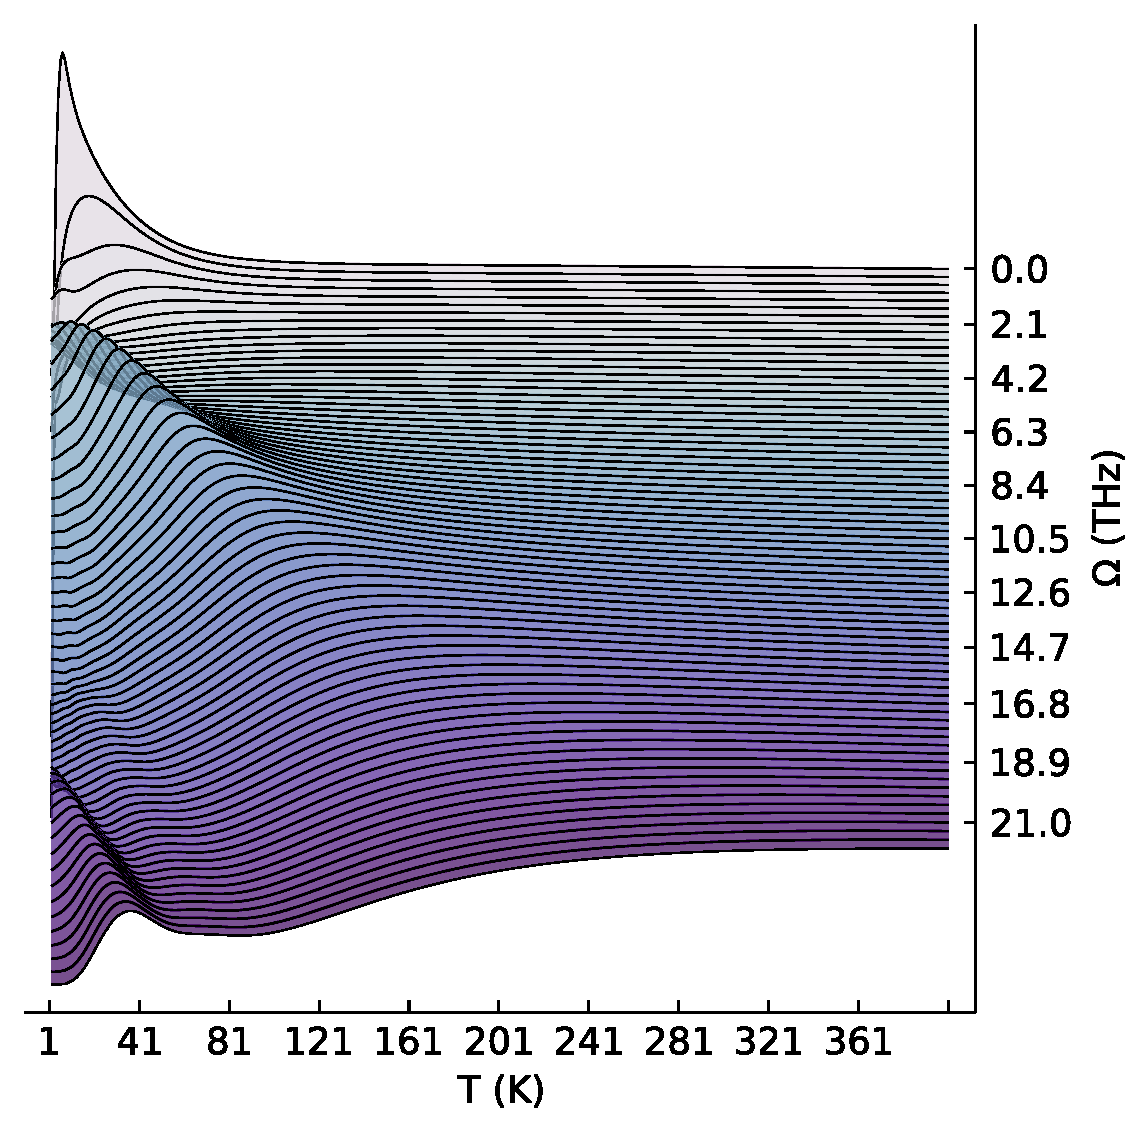
\includegraphics[width=.49\textwidth]{figures/multi_plot_freq_real.pdf}
    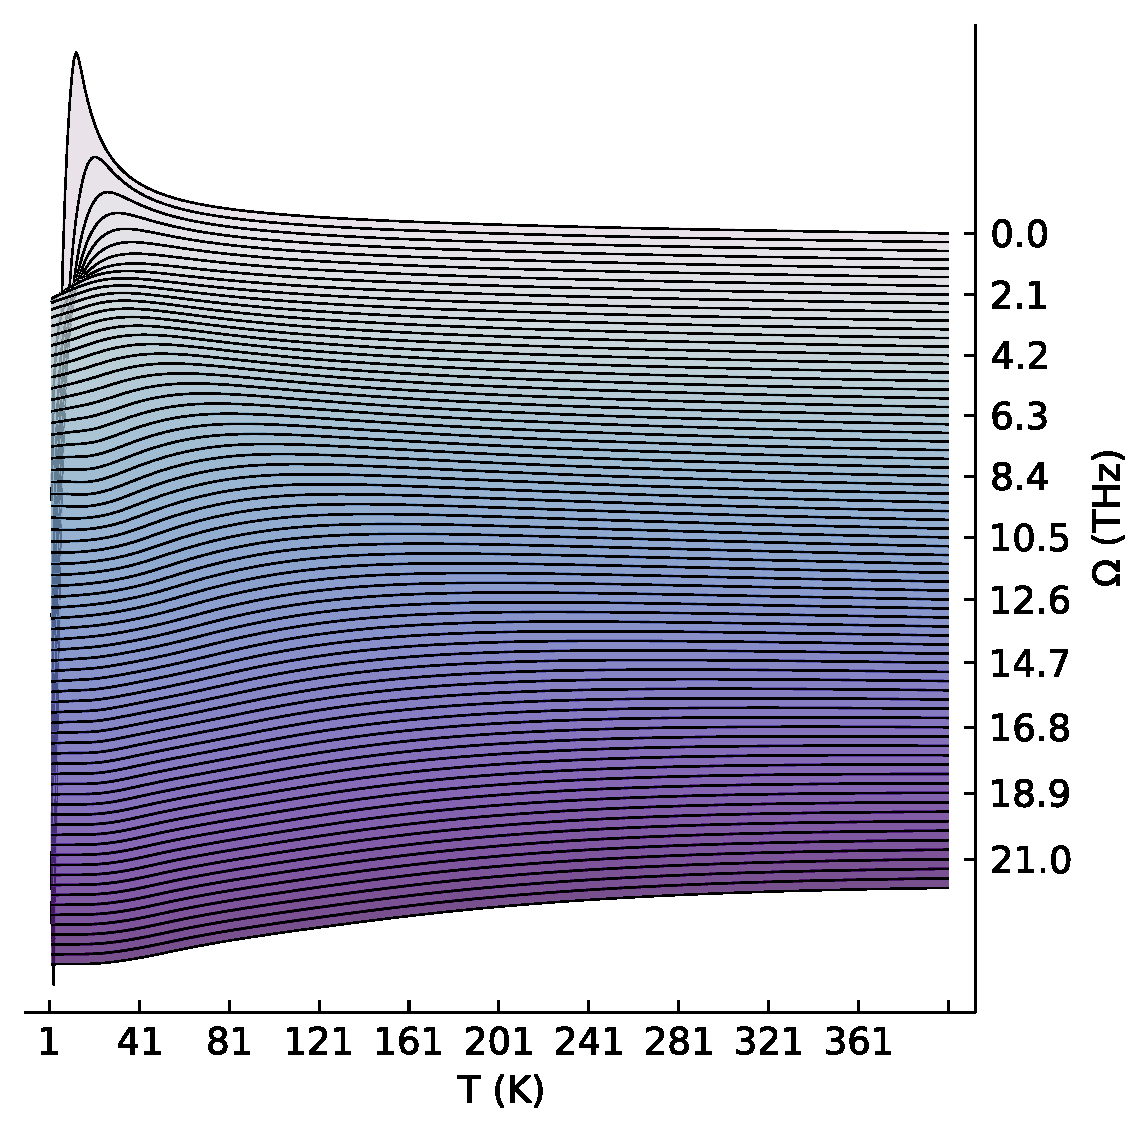
\includegraphics[width=.49\textwidth]{figures/A_plot_freq_real.pdf}
    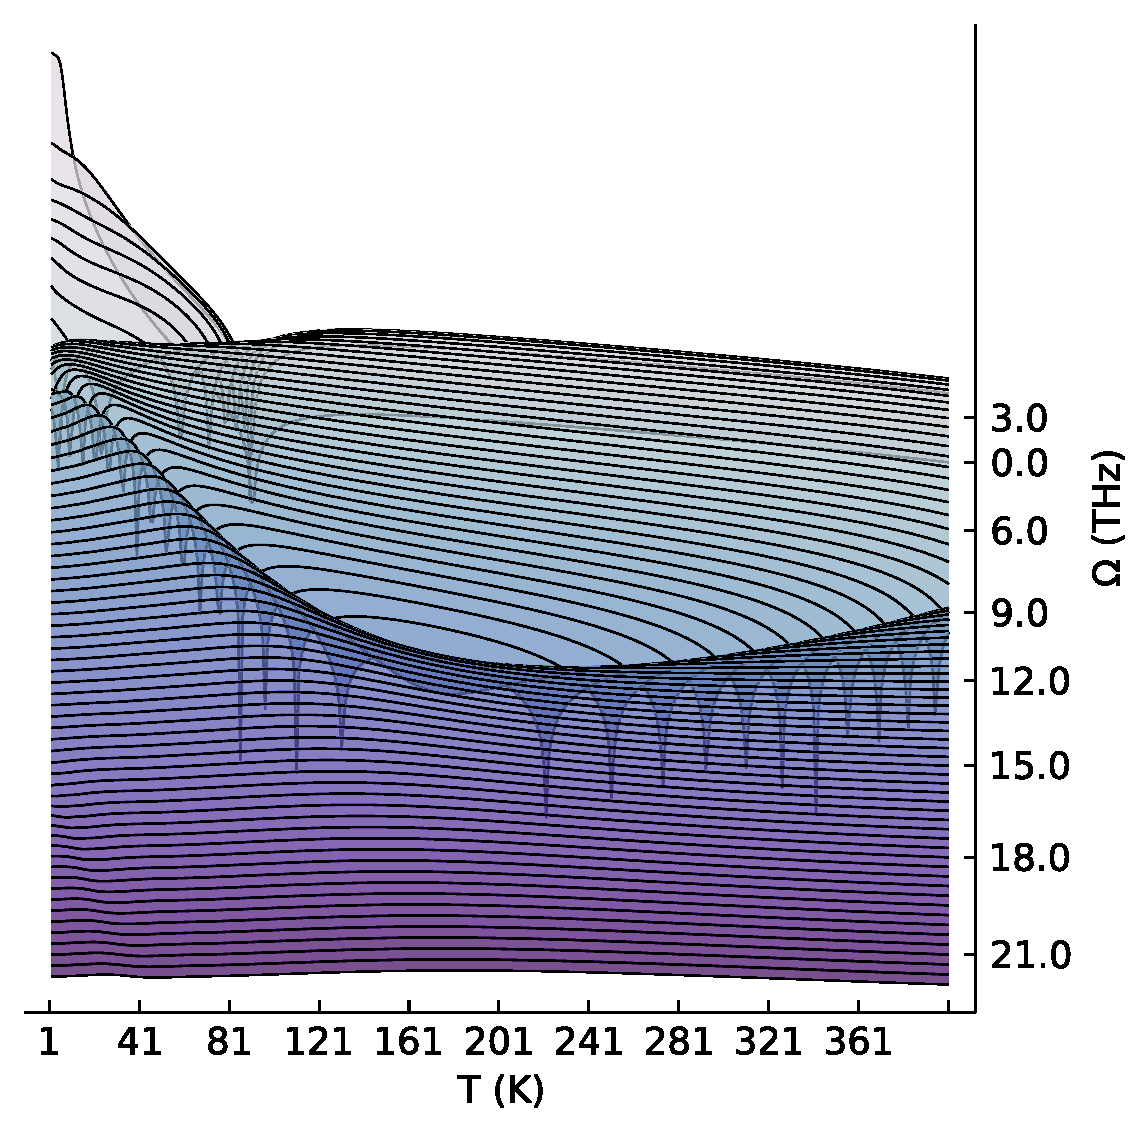
\includegraphics[width=.49\textwidth]{figures/multi_plot_freq_imag.pdf}
    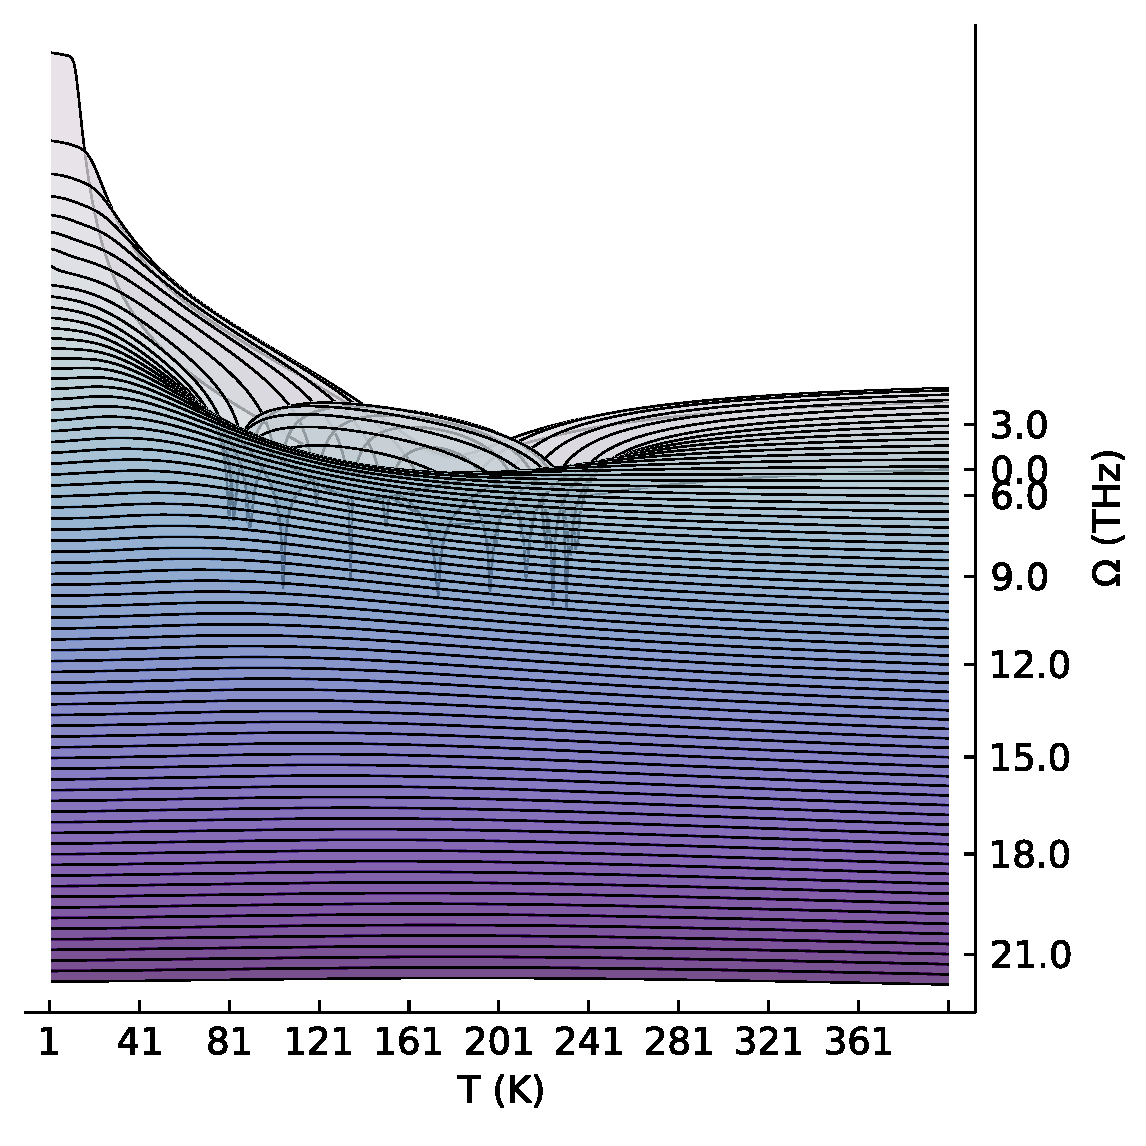
\includegraphics[width=.49\textwidth]{figures/A_plot_freq_imag.pdf}
    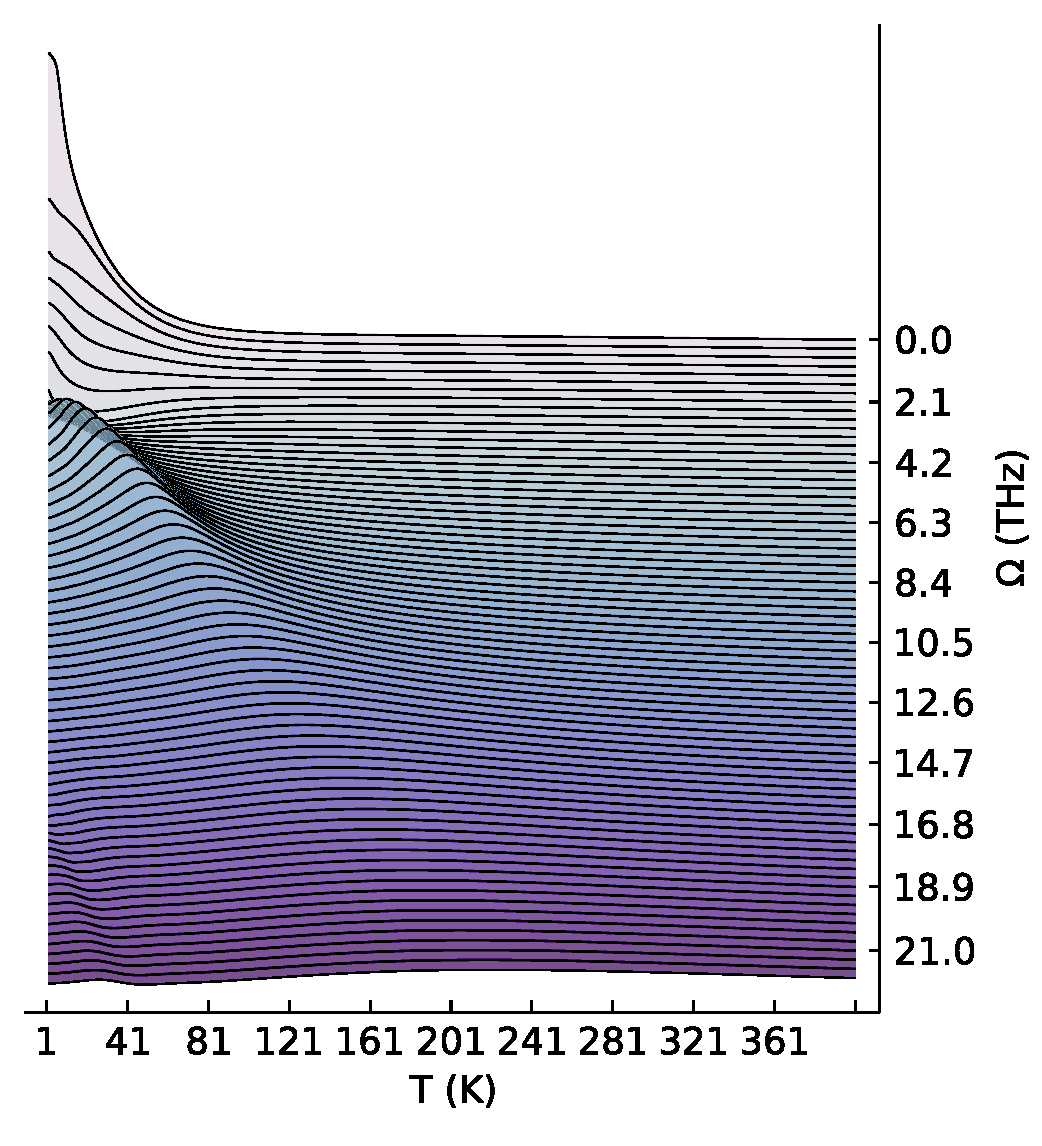
\includegraphics[width=.49\textwidth]{figures/multi_plot_freq_abs.pdf}
    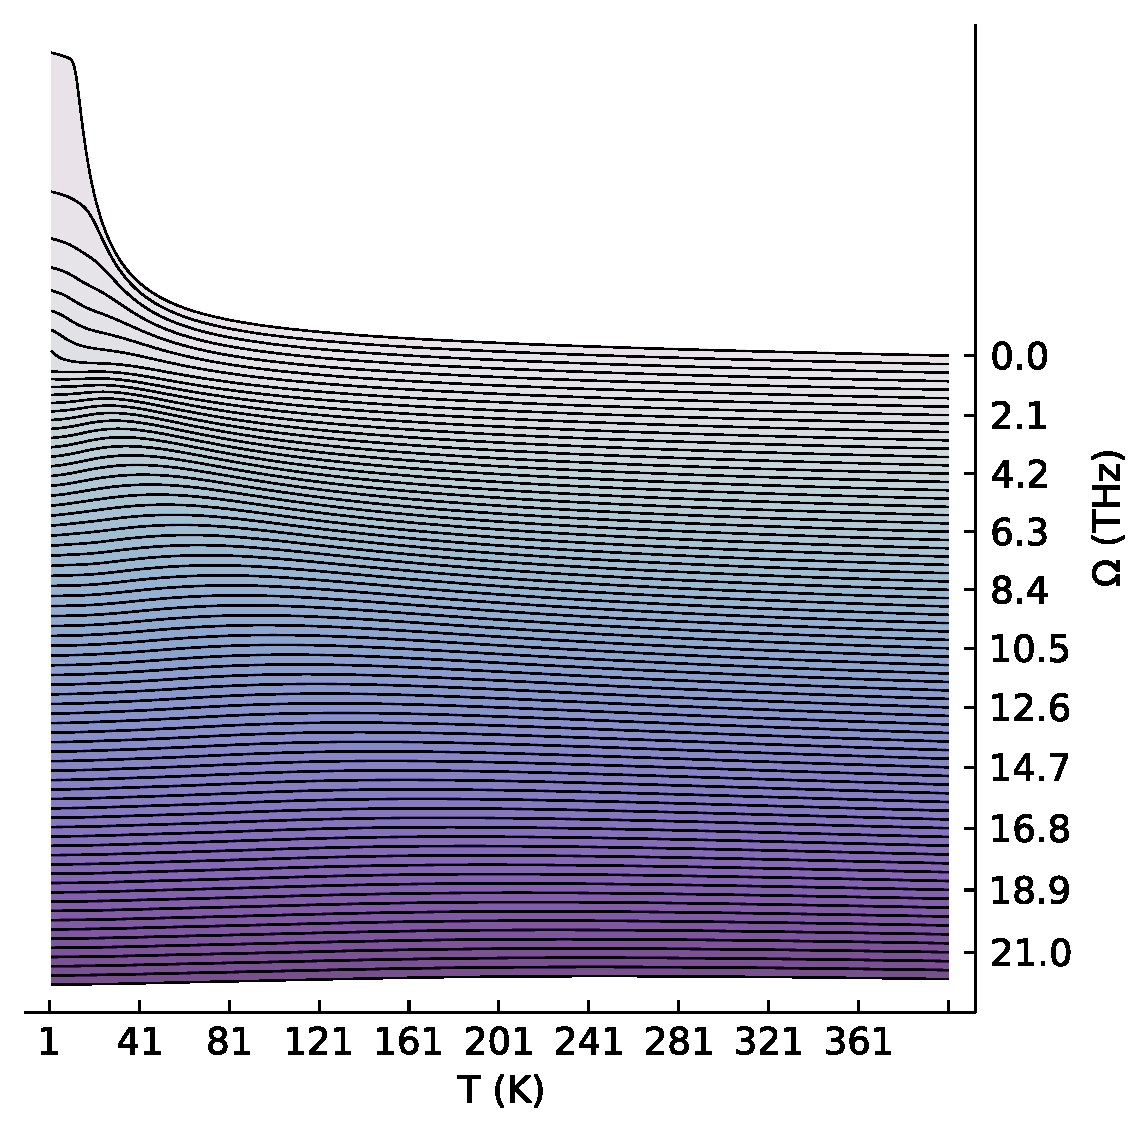
\includegraphics[width=.49\textwidth]{figures/A_plot_freq_abs.pdf}
    \caption{(a) Multiple phonon real conductivity. (b) A scheme real conductivity. (c) Multiple phonon imaginary conductivity. (d) A scheme imaginary conductivity. (e) Multiple phonon absolute conductivity. (f) A scheme absolute conductivity.}
\end{figure}

\subsection{Modelling terahertz spectroscopy unveiled polaron photoconductivity dynamics in Metal-Halide Perovskites}

\begin{figure}[t]
    \centering
    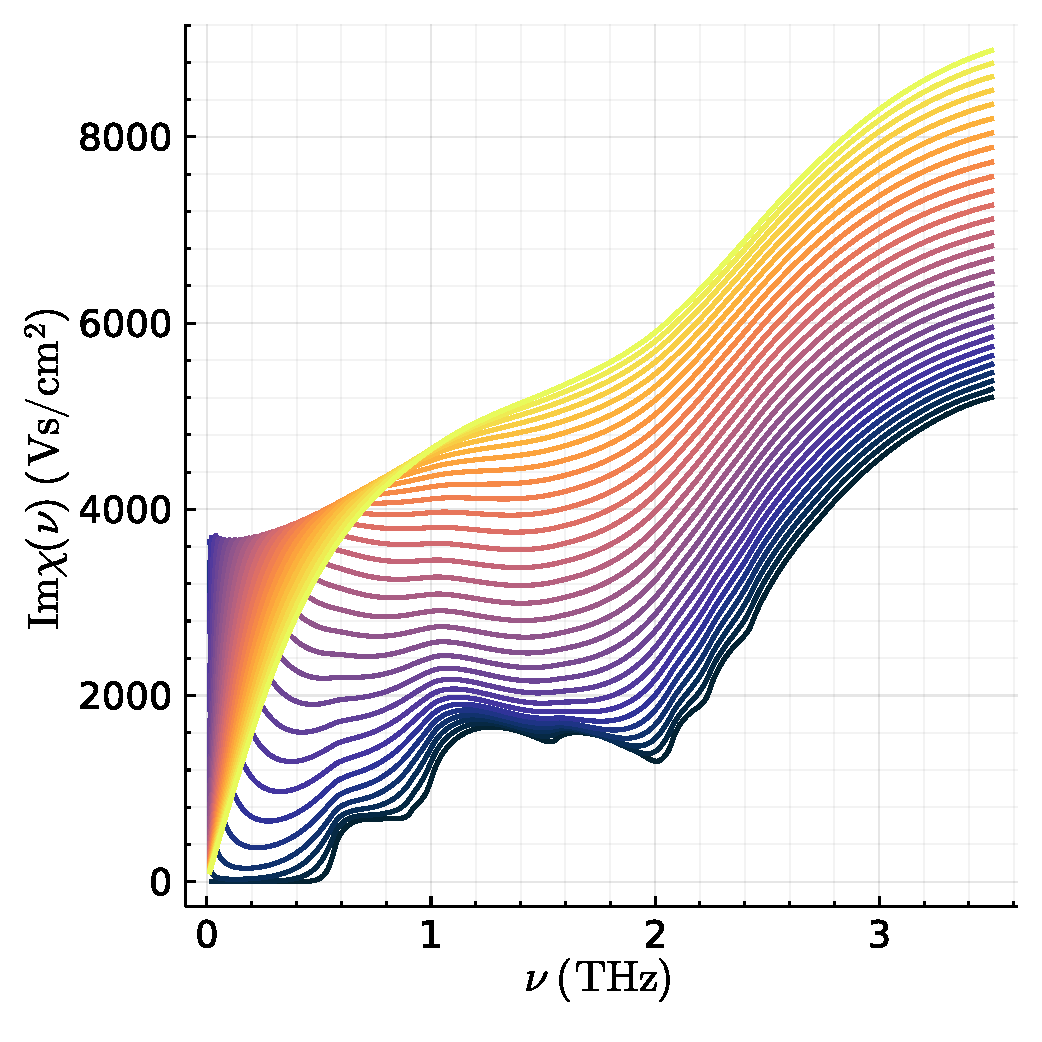
\includegraphics[width=.49\textwidth]{figures/zero_mem.pdf}
    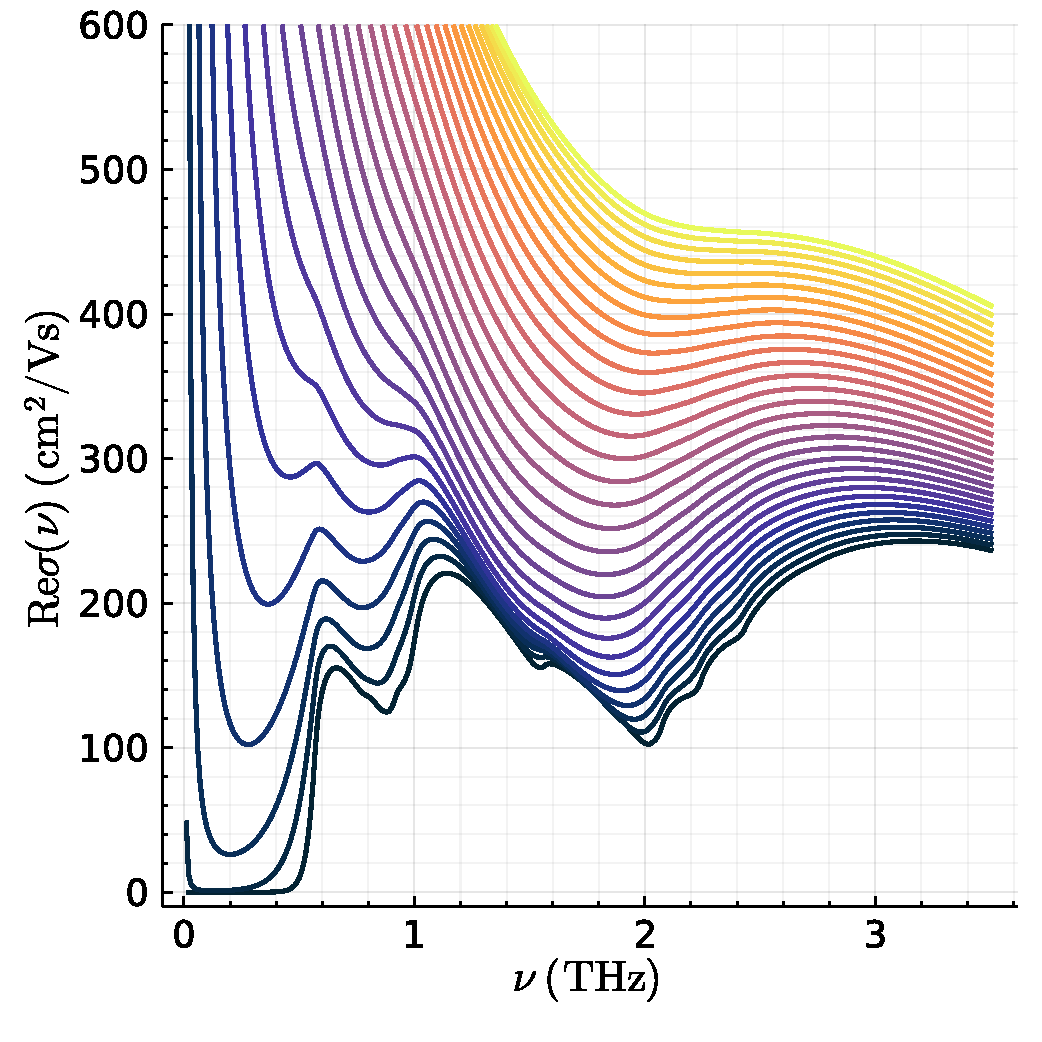
\includegraphics[width=.49\textwidth]{figures/zero_conduct.pdf}
    
    \caption{(left): The imaginary part of the multiple phonon mode memory function in Eq. (\ref{eqn:multi_memory}) evaluated for MAPbI$_3$. (right): The real part of the multiple phonon mode complex conductivity (i.e. mobility) in Eq. (\ref{eqn:freq_dep_mobility}) evaluated for MAPbI$_3$. These are calculated for the phonon modes listed in Table 1. The reduced thermodynamic beta $\beta_j = \hbar \omega_j / (k_B T)$ is evaluated for temperatures $T = 1$ K (black curves) to $T = 30$ K (yellow curves).}
    \label{fig:athermal_thz}
\end{figure}

Recently, we used used ultrafast visible pump-infrared push-terahertz probe spectroscopy to measure the real-time photo-conductivity of methyl-ammonium lead iodide in~\cite{zheng_multipulse_2021}. In this paper, I provided my multiple phonon mode mobility, applied to the $15$ modes of MAPbI$_3$ in Table 1, to model the complex conductivity and compare the results to the photo-conductivity measurements. 

\begin{figure}[t]  
    \centering
    \includegraphics[width=.7\textwidth]{figures/thz_plot.pdf}
    
    \caption{Terahertz photo-conductivity spectra obtained from a visible pump-IR push-THz probe measurement in~\cite{zheng_multipulse_2021}. The plot shows the real (solid markers) and imaginary (hollow markers) parts of the complex conductivity in MAPbI$_3$. The blue, black and green dashed-lines show before, at and after the arrival of the push pulse, respectively.}
    \label{fig:thzplot}
\end{figure}

In Figure \ref{fig:athermal_thz} I provide the low-temperature ($T = 1$ 
K to $T = 30$ K) results of the imaginary component of the memory function $\text{Im}\chi(\nu)$ (left) and the real part of the complex conductivity $\text{Re}\sigma(\nu)$ (right). These have peaks that occur around the frequencies $0.60$ THz, $1.25$ THz and $1.75$ THz, as well as a very broad peak that starts around $2.00$ THz that seems to have extra peaks underlying it to give the appearance of oscillations around $2.15$ THz and $2.25$ THz. 

From Figures \ref{fig:multicontour} and \ref{fig:multiridge} we see that the broad peak is the last feature which decays away at higher frequencies. The broad peak has a maximum around $3.00$ THz at $T = 1$, which flattens and shifts to higher frequencies at higher temperatures where it becomes the only remaining feature. This is to be compared to the photo-conductivity measurements shown in Figure \ref{fig:thzplot}, where the real component maxima occur around the frequencies $1.25$ THz and $2.25$ THz, with a shoulder occur on the side of the $1.25$ THz peak around $0.60$ THz. The shoulder and $1.25$ THz peak seem to be in agreement with the multiple phonon model, however the broader peak, whilst roughly around the right frequency of $2.25$ THz, is far broader and prominent in the theoretical model compared to the photo-conductivity measurements. 

One thing to note is the apparent temperature differences between the multiple phonon model and the experiment. In the multiple phonon model, the one-phonon peaks associated with each phonon mode only appear at very low-temperatures and are quickly washed out as the temperature increases until at around $T > 10$ K, only the broad peak around $3.00$ Thz remains. In the multiple phonon theory, it is assumed that the electron and phonon thermal-bath are at thermal equilibrium. However, in the experiment the electron(s) is definitely not at thermal equilibrium and is very hot.

\begin{figure}[h]
    \centering
    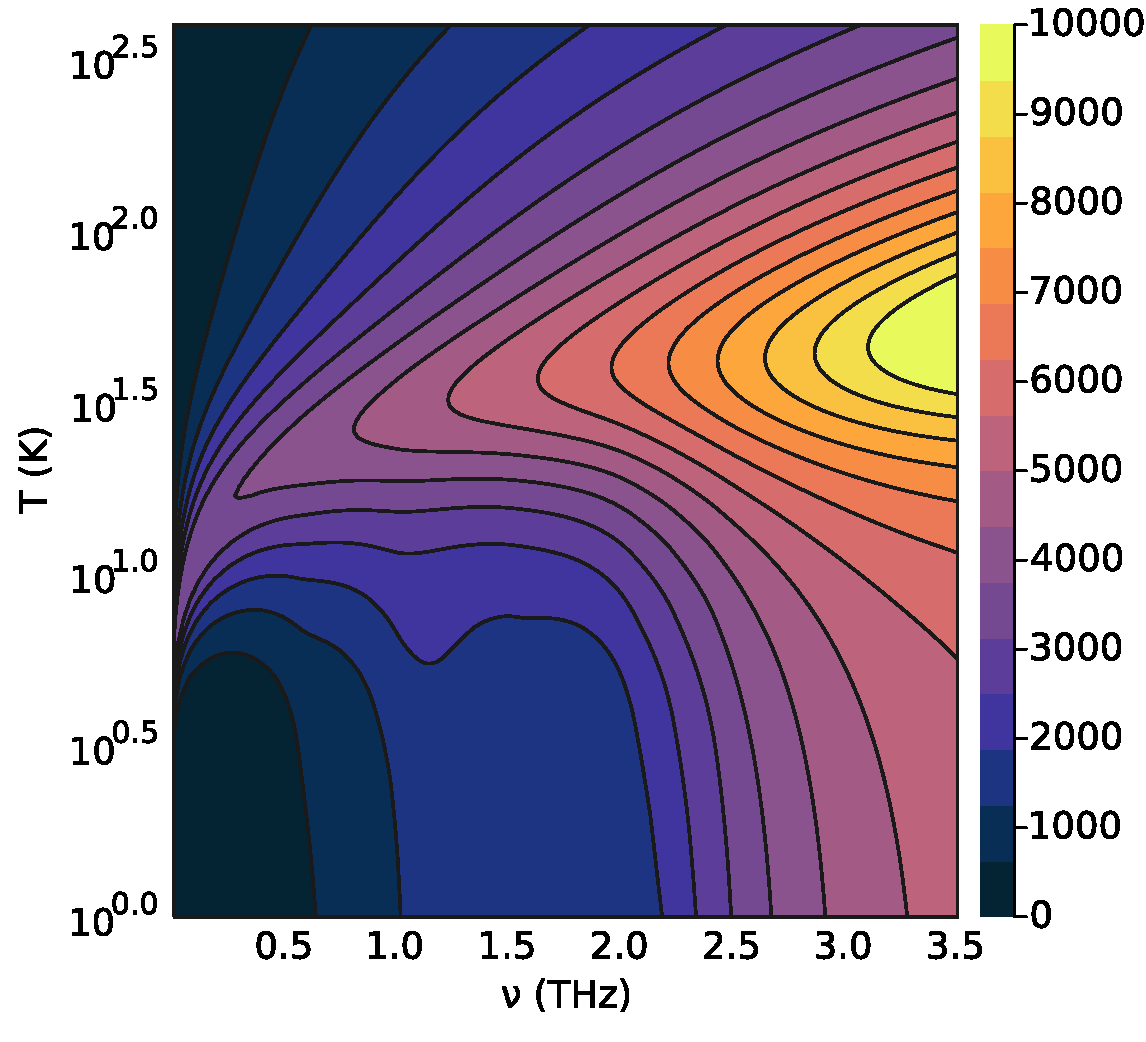
\includegraphics[width=.49\textwidth]{figures/multi_contour_real_chi.pdf}
    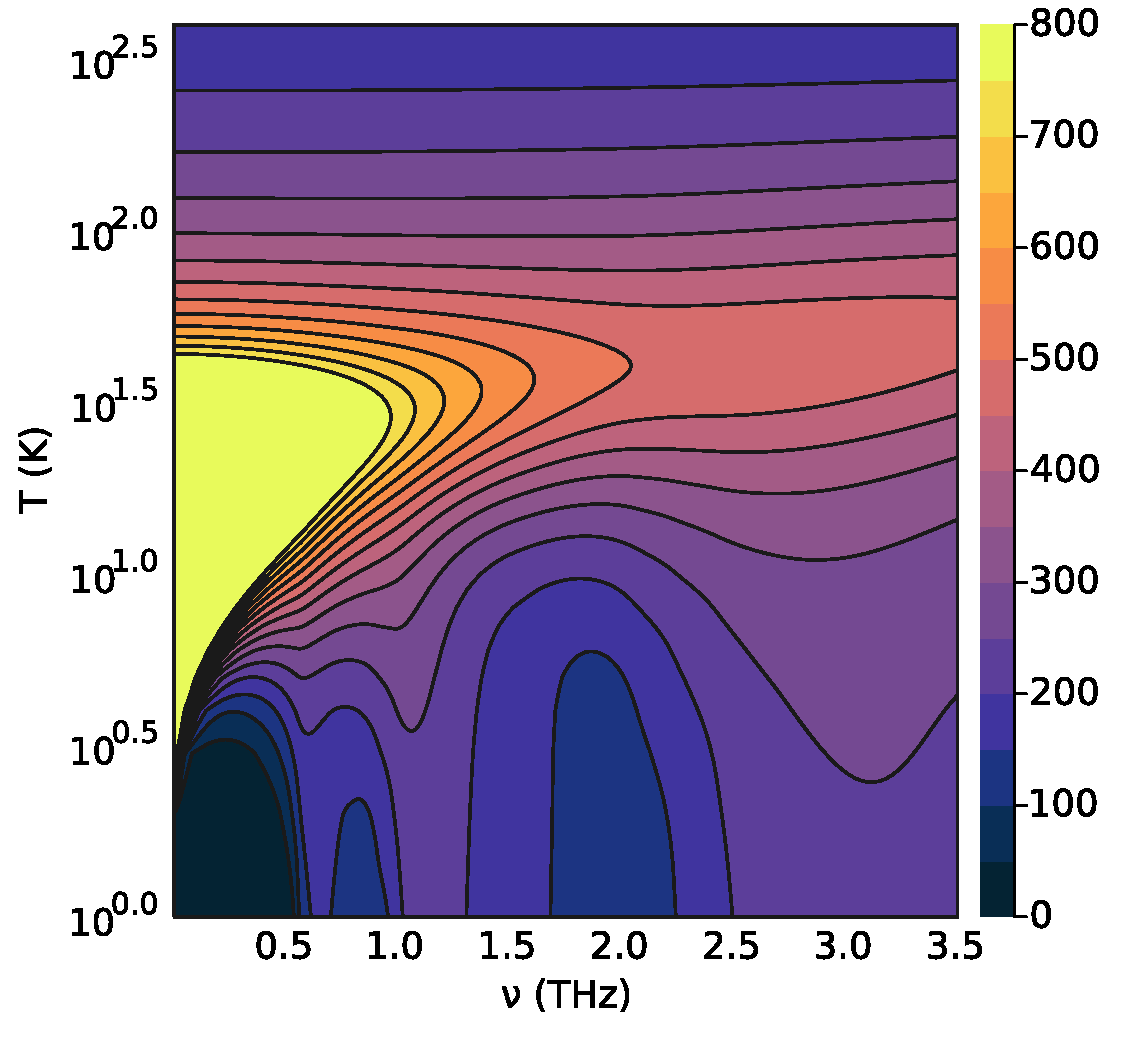
\includegraphics[width=.49\textwidth]{figures/multi_contour_real_0.pdf}
    
    \caption{Contour plots for (left): The imaginary part of the multiple phonon mode memory function (\ref{eqn:multi_memory}) evaluated for MAPbI$_3$. (right): The real part of the multiple phonon mode complex conductivity (\ref{eqn:freq_dep_mobility}) evaluated for MAPbI$_3$. Here the temperature axis is log-scaled and ranges from $T = 1$ K to $T = 400$ K and frequency zoomed in onto the range $\nu = 0$ THz to $\nu = 3.5$ THz.}
    \label{fig:thermal_thz}
\end{figure}

\section{Rubrene \& Organic Crystals}
\label{sec:chap-sixth-second}

\begin{figure}[!tbp]
    \centering
  \begin{subfigure}[b]{0.49\textwidth}
    \centering
    \includegraphics[width=\textwidth]{figures/rubrene_F_temp.png}
    \label{fig:rubrene_F_temp}
  \end{subfigure}
  \hfill
  \begin{subfigure}[b]{0.49\textwidth}
    \centering
    \includegraphics[width=\textwidth]{figures/rubrene_vw_temp.png}
    \label{fig:rubene_vw_temp}
  \end{subfigure}
  \begin{subfigure}[b]{0.49\textwidth}
    \centering
    \includegraphics[width=\textwidth]{figures/rubrene_mobility_temp_plot.png}
    \label{fig:rubrene_mobility_temp}
  \end{subfigure}
  \hfill
  \begin{subfigure}[b]{0.49\textwidth}
    \centering
    \includegraphics[width=\textwidth]{figures/rubrene_cond_freq.png}
    \label{fig:rubrene_cond_freq}
  \end{subfigure}
  \caption{Polaron properties of the variational Holstein model for a bulk 3D Rubrene organic crystal. \textbf{Top-left:} The polaron free energy $F$ (meV) in Rubrene as a function of temperature (K). \textbf{Top-right:} Optimal variational parameters $v$ and $w$ (THz2$\pi$) as a function of temperature (K). There appears to be some possible numerical artefact manifesting as the step-like increments. \textbf{Bottom-left:} The DC polaron mobility $\mu(T)$ (cm$^2$ V$^{-1}$ s$^{-1}$) as a function of temperature $T$ (K). \textbf{Bottom-right:} The real component of the conductivity $\Re\sigma(\Omega)$ (mS) as a function of frequency $\Omega$ (THz) for temperatures $T = 0.1$ K, $0.8$ K, $6.3$ K and $50$ K.}
  \label{fig:rubrene}
\end{figure}

In organic electronic materials it is understood that the charge-carrier state is a small polaron.  This is often modelled with semi-classical transfer rate theories as a classical object hopping from site to site. The matrix elements which parameterise these rate equations can be calculated, within certain approximations, from electronic-structure calculations, but it is a challenge (and often input to the simulation and calculations) to define the sites on which the charge carriers are localised. 
\newline

One of the prototypical materials studied frequently to investigate electron-phonon coupling is Rubrene (5,6,11,12-tetraphenyltetracene) which has one of the highest carrier mobilities and can reach few tens of cm$^2$/Vs for holes. This serves as a good test for applying our newly derived variational Holstein model to for predicting its charge-carrier mobility in bulk. I take parameters for Rubrene from Ordejon et al. \cite{Ordejn2017} where they derived Peierls (off-site) and Holstein (on-site) contributions by fitting the generalise Holstein-Peirels model with Density Functional Theory (DFT) calculations performed using SEISTA code. Here I make use of their Holstein parameters coupling, which I have listed in Table 1, and use these parameters within our newly derived variational Holstein method. For simplicity I consider a single effective phonon frequency, though the method presented here could be extended to multiple phonon modes, as I have demonstrated for the Fr\"ohlich Hamiltonian \cite{Martin2022}.
\newline

The results for ground-state Holstein and Fr\"ohlich polarons for Rubrene are shown in Table 2. Likewise, Table 3 gives the result for $T = 300$ K including the finite temperature DC mobility, which I calculate to be $\mu^{(H)}_{\text{Rubrene}} = 11.55$ cm$^2$V$^{-1}$s$^{-1}$ for the Holstein polaron and $\mu^{(F)}_{\text{Rubrene}} = 89.76$ cm$^2$V$^{-1}$s$^{-1}$ for the Fr\"ohlich polaron. Immediately, the Holstein prediction is inline which whats observed in experiments whereas the Fr\"ohlich greatly overestimates. Note that for the Fr\"ohlich model I have used an approximate comparative unitless coupling value of $\alpha^{(F)} \approx 3.0 \times \alpha^{(H)} = 1.785$.
\newline

\begin{table}
    \centering
    \begin{tabular}{|c|c|c|c|c|c|c|c|}
    \hline
        $g$ (meV) & $\omega_0$ (THz) & $J$ (meV) & $a$ (Å) & $\gamma$ & $m_b$ ($m_e$) & $\lambda^2$ & $\alpha$ \\
    \hline
         $106.8$ & $5.768$ & $134.0$ & $14.06$ & $0.178$ & $0.144$ & $20.04$ & $0.595$ \\
    \hline
    \end{tabular}
    \caption{3D Rubrene Bulk crystal data. Here $g$ is the Holstein hole-phonon coupling element, $\omega_0$ is the single-mode effective phonon frequency, $J$ is the electron transfer/hopping integral, $a$ is the geometric-meaned crystal lattice constant, $\gamma$ is the Holstein adiabaticity unitless parameter, $m_b$ is the effective hole band-mass, $\lambda^2 = (g / \hbar\omega_0)^2$ is the unitless squared hole-phonon coupling element and $\alpha = \lambda^2 \gamma / 6$ is the 3D unitless Holstein electron-phonon parameter.}
    \label{tab:rubrene}
\end{table}

At zero temperature, the Holstein polaron radius $R_0$ is $0.058$ times the lattice constant and so is definitely a \emph{small} polaron. Compare this to the Fr\"ohlich model where the polaron radius is $3.436$ times the lattice constant and so is a \emph{large} polaron. The Holstein polaron mass $M_0$ is only slightly large at $1.08$ times the hole band-mass, whereas the Fr\"ohlich polaron mass is already $2.48$ times heavier than the valence-band hole. Notably, the spring-constant $\kappa_0$ for the Holstein polaron is over $7$ times stronger than for the Fr\"ohlich polaron, which may correspond to an increased likelihood for the Holstein polaron to stay local to its current lattice site compared to the Fr\"ohlich polaron which is more delocalised and likely to move around. This is certainly reflected in the predicted room-temperature mobilities as mentioned above.
\newline

\begin{table}
    \centering
    \begin{tabular}{|c|c|c|c|c|c|c|}
    \hline
        & $v_0$ (THz$2\pi$) & $w_0$ (THz$2\pi$) & $M_0$ ($m_e$) &  $\kappa_0$ (mN m$^{-1}$) & $R_0$ (Å) & $F_0$ (meV) \\
    \hline
         Holstein & $3.376$ & $3.139$ & $0.157$ & $24.71$ & $0.828$ & $-0.178$ \\
    \hline
         Fr\"ohlich & $3.213$ & $2.758$ & $0.357$ & $3.250$ & $48.33$ & $-43.60$ \\
    \hline
    \end{tabular}
    \caption{Ground-state polaron properties for a Rubrene Bulk crystal calculated using the variational Holstein and Fr\"ohlich models.}
    \label{tab:rubrenegs}
\end{table}

\begin{table}
    \centering
    \begin{tabular}{|c|c|c|c|c|c|c|c|}
    \hline
        & $v$ (THz$2\pi$) & $w$ (THz$2\pi$) & $M$ ($m_e$) &  $\kappa$ (mN m$^{-1}$) & $R$ (Å) & $F$ (meV) & $\mu$ (cm$^2$V$^{-1}$s$^{-1}$) \\
    \hline
         Holstein & $4.656$ & $3.875$ & $0.444$ & $106.8$ & $1.465$ & $-3.735$ & $11.55$ \\
    \hline
        Fr\"ohlich & $8.143$ & $6.780$ & $0.442$ & $24.33$ & $83.07$ & $-81.58$ & $89.76$ \\
    \hline
    \end{tabular}
    \caption{Room temperature ($300$ K) polaron properties for a Rubrene Bulk crystal calculated using the variational Holstein and Fr\"ohlich models.}
    \label{tab:rubrenert}
\end{table}

At room-temperature $T = 300$ K the both polarons have roughly doubled in size. The Holstein polaron radius is still only $0.1$ times the lattice constant, whereas the Fr\"ohlich polaron is now about $6$ times larger than the lattice constant. Both polarons now have the same mass around $3$ times heavier than the valence-band hole. The spring-constant for the Holstein polaron is now only $4$ times greater than the Fr\"ohlich polaron.
\newline

In Figs. (\ref{fig:rubrene}) I give the temperature-dependent properties for the Rubrene polaron: polaron free energy and mobility. I also provide the optimal variational parameters $v$ and $w$ with respect to temperature.  Additionally, I provide the frequency-response of the optical conductivity at temperatures $T = 0.1$ K, $6.3$ K and $50$ K for the Holstein polaron and $T = 0.4$ K, $26$ K and $207$ K for the Fr\"ohlich polaron. The reason for the difference temperatures is so that the two models are within the same temperature regime for their respective inverse thermodynamics temperatures. For the Holstein polaron, $T^{(H)} = 1$ in polaron units is about $T = 11.6$ K, whereas in the Fr\"ohlich polaron units $T^{(F)} = 1$ is about $T = 48$ K. In the top-left figure we have the polaron free energies for Rubrene, which has a maximum at $T = 1$ in polaron units (note the figure shows the negative of the free energy). The Holstein polaron free energy is significantly smaller than the Fr\"ohlich polaron since it only ever couples to one lattice site, whereas the Fr\"olich polaron (in principle) couples to many lattice sites over an extent of multiple lattice constants. The Holstein polaron seems to have a sharper dependence on temperature at lower temperatures, but both polarons have a similar dependence above the Debye temperature $T_D \sim 120$ K corresponding to the energy of the Rubrene effective phonon mode. In the top-right figure we have the temperature-dependence of the $v$ and $w$ variational parameters. For both polarons these take a minimum at $T=1$ is the respective polaron units, but whilst above the Debye temperature $v$ and $w$ increase linearly with temperature for the Fr\"ohlich polaron, they reach a sudden plateau for the Holstein polaron. In the bottom-right figure we have the temperature-dependence of the polaron charge-carrier mobility. The Holstein polaron mobility descends far more quickly than for the Fr\"ohlich polaron and reaches what will eventually become a constant value around $\mu \sim 9.0$ cm$^2$V$^{-1}$s$^{-1}$ towards higher temperatures, whereas the Fr\"ohlich mobility will continue to decrease at a rate proportional to $\mu \sim T^{-1/2}$. Finally, the bottom-right figure show the frequency-dependence of the real-component of the complex conductivity for both polarons. At low temperatures both polarons see a response peak beginning at the phonon frequency $\omega_0 = 5.768$ THz, but then the Fr\"ohlich polaron response decays far more rapidly with frequency than the Holstein polaron. As we increase the temperature, this trend continues, except that for both polarons we begin to see some response below the phonon frequency due to presence of thermally excited phonons that generate an extra background response. This results in a local minimum in the conductivity around the effective polaron frequency $v$ as energy is lost to internal phonons that make up the polaron state. At much higher temperatures, the thermally excited phonon response now drowns out any kind of polaronic response and we are left with a typical Drude-like conductivity for both polarons, again with the Holstein polaron decaying more slowly than the Fr\"ohlich polaron with increasing frequency.

By applying both polaron models to Rubrene, we can more clearly see that the physics described by either model is very different. However, the predictions of the Holstein model seems to better align with the experimentally observed charge-carrier mobility.

\section{Cubic \& Anisotropic Materials}
\label{sec:chap-sixth-third}

\begin{figure}[t]
    \centering
    \includegraphics[width=.49\textwidth]{figures/ff_zpr.pdf}
    \includegraphics[width=.49\textwidth]{figures/ff_emass.pdf}
    
    \caption{Both figures are taken from~\cite{guster_frohlich_2021}. (left): The relative differences between the ground-state energy of the polaron determined using perturbation theory (which fully accounts for any anisotropy) and the Feynman variational approach (using my approximate treatment of anisotropy). (right): The relative difference between the effective masses determined using perturbation theory and the Feynman variational approach (again only approximately accounting for anisotropy). $m^*_{P, iso}$ is the isotropic effective mass, $m^*_{P, \perp}$ and $m^*_{P, z}$ are the in-plane and out-of-plane polaron effective masses.}
    \label{fig:anisotropy}
\end{figure}

In~\cite{guster_frohlich_2021}, we investigate the polaron effective mass, radius and ground-state energy that arise from a generalised Fr\"ohlich Hamiltonian that incorporates degenerate bands with anisotropy and multiple phonon branches. These polaron properties are calculated for 20 cubic materials (including II-VI compounds: CdS, CdSe, CdTe, ZnS, ZnSe, ZnTe; III-V compounds: AlAs, AlSb, AlP, BAs, BN, GaAs, GaN, GaP; oxides: BaO, CaO, Li$_2$O, MgO, SrO; and SiC) using the lowest order of perturbation theory and the strong coupling limit. \newline

In the non-degenerate case, I provide a na\"ive extension of Feynman's path integral approach to include anisotropic effective band masses which is used as a point of comparison with the full perturbative treatment for characterising the polaron in the weak-coupling limit (c.f. section IIb in~\cite{guster_frohlich_2021} and subsection 3.8 of this chapter). From Figure \ref{fig:anisotropy} (left) we see that the variational approach gives a lower estimate for the ground-state compared to the perturbative result for both isotropic (up to $2.5$\% lower) and anisotropic (up to $17.5$\% lower) materials. In Figure \ref{fig:anisotropy} (right), we have the relative difference in polaron effective mass between the two approaches. The largest difference is found in materials that, within the Fr\"ohlich approach, are found in~\cite{guster_frohlich_2021} to be at the continuum limit breakdown where the discrete nature of the lattice cannot be ignored. These materials include BaO, CaO, SrO and, to a lesser extent, Li$_2$O. In both the anisostropic and isotropic cases the relative difference increases with polaron effective mass, and the in-plane and out-of-plane effective mass differences seem to diverge. This sudden increase in the relative difference is associated with a breakdown limit around $\alpha = 6$ in the perturbative approach for determining the polaron effective mass.

\section{High-Throughput Material Classification}
\label{sec:chap-sixth-fourth}